% =====================================================================
%  magex: magnetic exchange from Wannier Hamiltonians -- theory & code
%  Compile:  pdflatex magex_theory.tex   (twice)    figures in ./figs/
% =====================================================================
\documentclass[aspectratio=169,9pt]{beamer}
\usetheme[progressbar=frametitle,numbering=fraction,block=fill]{metropolis}
\usepackage[T1]{fontenc}
\usepackage{amsmath,amssymb,bm,mathtools}
\usepackage{booktabs,tabularx,array,multirow}
\usepackage{tikz}
\usetikzlibrary{arrows.meta,positioning,calc,decorations.pathreplacing,decorations.pathmorphing,shapes.geometric,shadows,fit,backgrounds,matrix}
\usepackage[most]{tcolorbox}
\usepackage{graphicx}

% ---------------------------------------------------------------------
%  Palette  (one colour per kind of quantity)
% ---------------------------------------------------------------------
\definecolor{navy}{HTML}{14203A}
\definecolor{paper}{HTML}{F8F6F0}
\definecolor{cH}{HTML}{2E8B57}   % Hamiltonian, exchange field X, p     (green)
\definecolor{cS}{HTML}{E67E22}   % spin-orbit coupling S, L.S             (orange)
\definecolor{cG}{HTML}{2E6DB4}   % Green's function, eigenvectors         (blue)
\definecolor{cJ}{HTML}{C0392B}   % exchange tensor J, D, A                (red)
\definecolor{cR}{HTML}{7D3C98}   % rotations, angles, axes, spin dirs     (purple)
\definecolor{cK}{HTML}{138D90}   % Hessians K, T, perturbations W         (teal)
\definecolor{cE}{HTML}{8E5B2E}   % energies Omega, f, mu, contour         (brown)
\definecolor{cM}{HTML}{B7950B}   % magnon / spin-wave quantities          (gold)
\definecolor{cC}{HTML}{4A5568}   % code, MPI                              (slate)
\definecolor{lgrey}{HTML}{EEF0F3}

\newcommand{\cH}[1]{{\color{cH}#1}}
\newcommand{\cS}[1]{{\color{cS}#1}}
\newcommand{\cG}[1]{{\color{cG}#1}}
\newcommand{\cJ}[1]{{\color{cJ}#1}}
\newcommand{\cR}[1]{{\color{cR}#1}}
\newcommand{\cK}[1]{{\color{cK}#1}}
\newcommand{\cE}[1]{{\color{cE}#1}}
\newcommand{\cM}[1]{{\color{cM}#1}}
\newcommand{\cC}[1]{{\color{cC}\texttt{#1}}}

% frequently used coloured symbols
\newcommand{\Hm}{\cH{H}}
\newcommand{\X}{\cH{X}}
\newcommand{\p}{\cH{\bm p}}
\newcommand{\SO}{\cS{S}}
\newcommand{\G}{\cG{G}}
\newcommand{\Psim}{\cG{\Psi}}
\newcommand{\J}{\cJ{J}}
\newcommand{\Dv}{\cJ{\bm D}}
\newcommand{\A}{\cJ{A}}
\newcommand{\e}{\cR{\bm e}}
\newcommand{\n}{\cR{\bm n}}
\newcommand{\ph}{\cR{\phi}}
\newcommand{\K}{\cK{K}}
\newcommand{\T}{\cK{T}}
\newcommand{\W}{\cK{W}}
\newcommand{\Om}{\cE{\Omega}}
\newcommand{\fF}{\cE{f}}
\newcommand{\mus}{\cE{\mu}}
\newcommand{\sig}{\bm\sigma}

\setbeamercolor{background canvas}{bg=paper}
\setbeamercolor{frametitle}{bg=navy,fg=white}
\setbeamercolor{progress bar}{fg=cS,bg=navy!40}
\setbeamercolor{alerted text}{fg=cJ}
\setbeamercolor{block title}{bg=navy!10,fg=navy}
\setbeamercolor{block body}{bg=white}
\setbeamerfont{frametitle}{size=\large,series=\bfseries}

% ---------------------------------------------------------------------
%  Boxes
% ---------------------------------------------------------------------
\newtcolorbox{eqbox}[2][]{enhanced,colback=white,colframe=#2,boxrule=0.6pt,arc=2pt,
  left=4pt,right=4pt,top=2pt,bottom=2pt,leftrule=3pt,fonttitle=\bfseries\small,
  coltitle=white,colbacktitle=#2,title={#1},attach boxed title to top left={yshift=-2mm,xshift=3mm},
  boxed title style={arc=1pt,boxrule=0pt}}
\newtcolorbox{plainbox}[1]{enhanced,colback=white,colframe=#1,boxrule=0.6pt,arc=2pt,
  left=4pt,right=4pt,top=3pt,bottom=3pt,leftrule=3pt}
\newtcolorbox{proofbox}[1][Proof]{enhanced,colback=lgrey,colframe=cC!70,boxrule=0.4pt,arc=2pt,
  left=5pt,right=5pt,top=2pt,bottom=2pt,fonttitle=\bfseries\small,title={#1},
  colbacktitle=cC!80,coltitle=white}
\newcommand{\cellfill}[3]{\fill[#3] (#1*1.1,2.2-#2*1.1) rectangle ++(1.0,1.0);}
\newcommand{\qedb}{\hfill$\blacksquare$}
\newcommand{\takeaway}[1]{\vfill\begin{tcolorbox}[enhanced,colback=navy,colframe=navy,coltext=white,arc=2pt,
  left=6pt,right=6pt,top=2pt,bottom=2pt]\small\textbf{Take-away:} #1\end{tcolorbox}}
\newcommand{\codeline}[1]{{\small\color{cC}\faCode}~\cC{#1}}
\providecommand{\faCode}{$\triangleright$}
\newcommand{\src}[1]{\hfill{\scriptsize\color{cC}\ttfamily magex/#1}}

\title{\textbf{magex}: magnetic exchange, anisotropy and magnons\\from Wannier Hamiltonians}
\subtitle{Green's-function theory, full derivations, and what every routine of the code does}
\author{Gokaran Shukla}
\institute{KAUST, Thuwal, Saudi Arabia}
\date{November 10, 2026}

\begin{document}

% =====================================================================
%  TITLE
% =====================================================================
{
\begin{frame}[plain]
\begin{tikzpicture}[remember picture,overlay]
  \shade[top color=navy,bottom color=navy!70!cG] (current page.north west) rectangle (current page.south east);
  % spin lattice
  \foreach \x in {0,...,7}{\foreach \y in {0,...,2}{
     \pgfmathsetmacro{\ang}{90+18*sin(40*\x+70*\y)}
     \fill[white!80!cR] ($(current page.south east)+(-6.2+0.75*\x,0.6+0.75*\y)$) circle (0.09);
     \draw[-{Stealth[length=2.2mm]},very thick,color=cS!80!white]
        ($(current page.south east)+(-6.2+0.75*\x,0.6+0.75*\y)$) -- ++(\ang:0.42);
  }}
  \node[anchor=north west,text width=12.5cm,white] at ($(current page.north west)+(0.8,-1.2)$)
   {{\LARGE\bfseries \textcolor{cS!80!white}{magex}}\\[3pt]
    {\Large Magnetic exchange, anisotropy and magnons\\ from Wannier Hamiltonians}\\[8pt]
    {\normalsize\color{white!80} Green's-function theory $\cdot$ full derivations $\cdot$ code walkthrough $\cdot$ validation}};
  \node[anchor=south west,white,text width=9cm] at ($(current page.south west)+(0.8,0.7)$)
   {\textbf{Gokaran Shukla}\\ \small KAUST, Thuwal\\ \small November 10, 2026};
\end{tikzpicture}
\end{frame}
}

\begin{frame}{Roadmap}
\begin{columns}[T]
\column{0.5\textwidth}
\begin{enumerate}\small
\item Goal: the extended Heisenberg model
\item Why a new code: limits of LKAG/TB2J
\item The tight-binding model and its spin decomposition
\item Magnetic force theorem \& Lloyd formula
\item Rigid rotations, Hessians, Green's functions
\item Energy integration with Ozaki poles
\item Rotational invariance: partitioning the exchange field
\end{enumerate}
\column{0.5\textwidth}
\begin{enumerate}\small\setcounter{enumi}{7}
\item Mapping to $\J$, $\Dv$, $\J^{\rm ani}$, $\A$ from one DFT run
\item Symmetrisation and supercell aliasing
\item Beyond MFT: Bruno renormalisation, ligand downfolding
\item Finite angles: Lloyd pair energies, biquadratic terms
\item Linear spin-wave theory
\item MPI implementation
\item Validation and physics results (SrMnO$_3$, bcc Fe, CrI$_3$)
\end{enumerate}
\end{columns}
\end{frame}

\begin{frame}{Colour code used throughout}
\centering
\renewcommand{\arraystretch}{1.35}
\begin{tabular}{>{\bfseries}l l l}
\toprule
colour & quantity & symbols \\
\midrule
\cH{green}  & Hamiltonian, exchange field & $\Hm,\ \cH{H_0},\ \X,\ \p_i,\ \cH{Y}$ \\
\cS{orange} & spin--orbit coupling & $\SO,\ \cS{\xi\,\bm L\cdot\bm S}$ \\
\cG{blue}   & Green's function, eigenstates & $\G,\ \Psim,\ \cG{\varepsilon_{n\bm k}},\ \cG{U_a}$ \\
\cJ{red}    & spin-model parameters & $\J,\ \Dv,\ \J^{\rm ani},\ \A$ \\
\cR{purple} & rotations and directions & $\e_i,\ \n_i,\ \ph,\ \cR{\mathcal R},\ \cR{\theta}$ \\
\cK{teal}   & Hessians, perturbations & $\K_{ab},\ \T_i,\ \W_{ia},\ \cK{D_i}$ \\
\cE{brown}  & energies, occupation, contour & $\Om,\ \fF,\ \mus,\ \cE{z_p},\ \cE{w_p}$ \\
\cM{gold}   & magnons & $\cM{\omega(\bm q)},\ \cM{b_i},\ \cM{h(\bm k)}$ \\
\cC{slate}  & code / MPI & \cC{engine.py}, \cC{Allreduce} \\
\bottomrule
\end{tabular}
\end{frame}

% =====================================================================
\section{Goal and motivation}
% =====================================================================
\begin{frame}{The target: an extended Heisenberg model}
\begin{columns}[c]
\column{0.58\textwidth}
\begin{eqbox}[Spin Hamiltonian (TB2J convention)]{cJ}
\[
E[\{\e\}]=\sum_i \e_i\!\cdot\!\A_i\!\cdot\!\e_i\;-\;\sum_{i\neq j}\e_i\!\cdot\!\J_{ij}\!\cdot\!\e_j
\]
\small unit spins $|\e_i|=1$; every ordered pair counted, $\J_{ji}=\J_{ij}^{T}$; $\J>0$ ferromagnetic.
\end{eqbox}
\begin{eqbox}[Decomposition of the $3\times3$ tensor]{cJ}
\[
\J_{ij}=\underbrace{\cJ{J^{\rm iso}_{ij}}\,\mathbb 1}_{\text{Heisenberg}}+\underbrace{\J^{\rm ani}_{ij}}_{\text{sym., traceless}}+\underbrace{\J^{A}_{ij}}_{\text{antisym.}}
\]
\[
-\e_i\!\cdot\!\J^{A}_{ij}\!\cdot\!\e_j=-\Dv_{ij}\!\cdot(\e_i\times\e_j),\quad
\Dv=(\cJ{J^A_{yz}},\cJ{J^A_{zx}},\cJ{J^A_{xy}})
\]
\end{eqbox}
\column{0.40\textwidth}
\centering
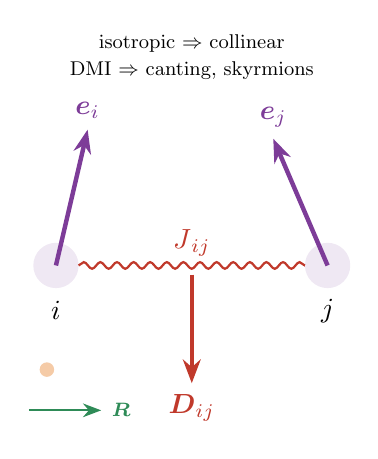
\begin{tikzpicture}[scale=1.15]
  \fill[cR!12] (0,0) circle (0.25); \fill[cR!12] (3,0) circle (0.25);
  \node at (0,-0.5) {$i$}; \node at (3,-0.5) {$j$};
  \draw[-{Stealth[length=3mm]},line width=1.6pt,cR] (0,0) -- (0.35,1.5) node[above]{$\e_i$};
  \draw[-{Stealth[length=3mm]},line width=1.6pt,cR] (3,0) -- (2.4,1.4) node[above]{$\e_j$};
  \draw[thick,cJ,decorate,decoration={snake,amplitude=1.2pt,segment length=6pt}] (0.25,0) -- (2.75,0);
  \node[cJ] at (1.5,0.25) {$\J_{ij}$};
  \draw[-{Stealth[length=3mm]},line width=1.4pt,cJ] (1.5,-0.1) -- (1.5,-1.3) node[below]{$\Dv_{ij}$};
  \draw[-{Stealth},thick,cH] (-0.3,-1.6) -- (0.5,-1.6) node[right]{\scriptsize $\bm R$};
  \fill[cS!40] (-0.1,-1.15) circle (0.08);
  \node[scale=0.8,align=center] at (1.5,2.3) {\small isotropic $\Rightarrow$ collinear\\ \small DMI $\Rightarrow$ canting, skyrmions};
\end{tikzpicture}
\end{columns}
\takeaway{every quantity the code prints is a coefficient of this energy function; the job is to extract all of them from one DFT Hamiltonian.}
\end{frame}

\begin{frame}{Two ways to get the parameters}
\begin{columns}[T]
\column{0.48\textwidth}
\begin{plainbox}{cC}
\textbf{Energy mapping}\\[2pt]
\small
\begin{itemize}
\item DFT for many spin configurations, large supercells
\item fit $\J$ to total energies
\item metallisation of high-energy states, supercell-dependent fits, many non-collinear SOC runs
\end{itemize}
\end{plainbox}
\column{0.48\textwidth}
\begin{plainbox}{cG}
\textbf{Green's function / force theorem (LKAG)}\\[2pt]
\small
\begin{itemize}
\item one ground-state calculation
\item $\J_{ij}$ at all distances from $\G_{ij}(\bm R)$
\item local linear response $\Rightarrow$ exact small-angle curvature of the band energy
\end{itemize}
\end{plainbox}
\end{columns}
\vspace{6pt}
\centering
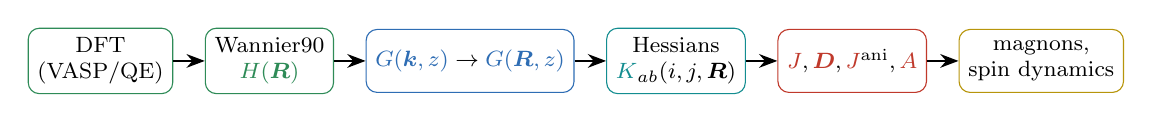
\begin{tikzpicture}[node distance=4mm and 4mm,box/.style={draw,rounded corners,fill=white,align=center,font=\footnotesize,minimum height=8mm}]
\node[box,draw=cH] (dft) {DFT\\(VASP/QE)};
\node[box,draw=cH,right=of dft] (w90) {Wannier90\\$\cH{H(\bm R)}$};
\node[box,draw=cG,right=of w90] (gf) {$\cG{G(\bm k,z)}\to\cG{G(\bm R,z)}$};
\node[box,draw=cK,right=of gf] (hess) {Hessians\\$\K_{ab}(i,j,\bm R)$};
\node[box,draw=cJ,right=of hess] (heis) {$\J,\Dv,\J^{\rm ani},\A$};
\node[box,draw=cM,right=of heis] (mag) {magnons,\\spin dynamics};
\draw[-Stealth,thick] (dft)--(w90); \draw[-Stealth,thick] (w90)--(gf); \draw[-Stealth,thick] (gf)--(hess);
\draw[-Stealth,thick] (hess)--(heis); \draw[-Stealth,thick] (heis)--(mag);
\end{tikzpicture}
\end{frame}

\begin{frame}{What limits the standard LKAG/TB2J implementation}
\footnotesize
\renewcommand{\arraystretch}{1.12}
\begin{tabularx}{\textwidth}{>{\raggedright\arraybackslash}p{0.43\textwidth} >{\raggedright\arraybackslash}X}
\toprule
\textbf{limitation} & \textbf{magex} \\
\midrule
only the \emph{on-site} exchange block is rotated; inter-atomic spin-dependent Wannier elements stay fixed $\Rightarrow$ no global rotation, Goldstone sum rule broken & \cH{weighted partition} of the full $\X(\bm R)$; sum rule exact; bcc Fe $J_1$: $9.5\to21.2$ meV \\
full tensor needs 3 DFT runs (x, y, z) and a merge & \cR{rotate $\X$ relative to the lattice} in one Hamiltonian \\
no single-ion anisotropy from Wannier input & $\A_i$ from on-site Hessians + band MAE cross-check \\
$T=0$ contour with user $E_{\min}$ & \cE{Ozaki poles} at finite $T$, no $E_{\min}$ \\
plain MFT & \cK{Bruno renormalisation} \\
ligand moments rigid/ignored & \cK{Schur-complement downfolding} \\
biquadratic from small angles "often unphysical" & exact \cE{Lloyd} finite-angle pair energies \\
Wannier noise unquantified & spglib symmetrisation; change reported \\
magnons isotropic only & LSWT with full $\J$, $\Dv$, $\A$ \\
\bottomrule
\end{tabularx}
\end{frame}

\begin{frame}{Code architecture}
\centering
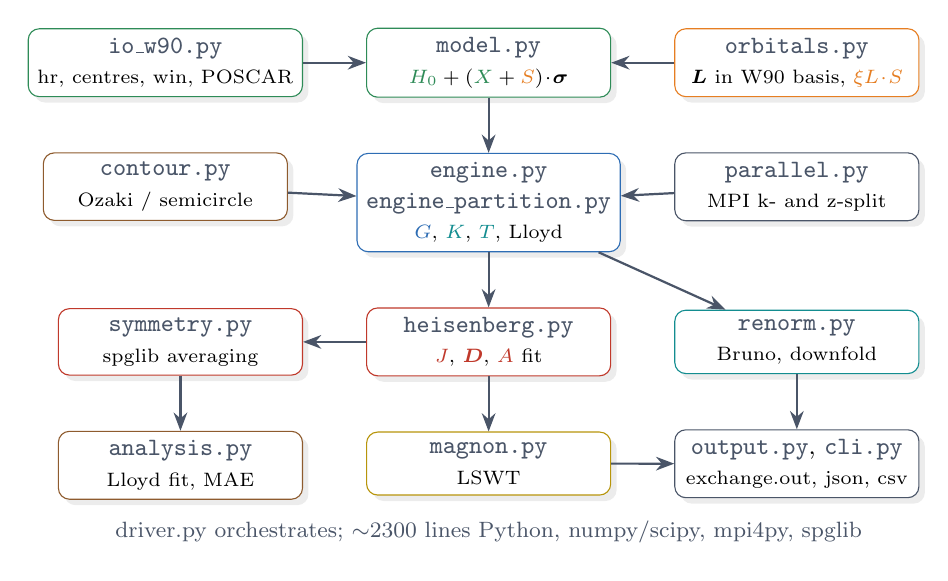
\begin{tikzpicture}[font=\small,
  m/.style={draw=cC,fill=white,rounded corners,minimum width=3.1cm,minimum height=8mm,align=center,drop shadow={opacity=0.15}},
  a/.style={-Stealth,thick,cC}]
\node[m,draw=cH] (io) {\cC{io\_w90.py}\\\scriptsize hr, centres, win, POSCAR};
\node[m,draw=cH,right=8mm of io] (model) {\cC{model.py}\\\scriptsize $\cH{H_0}+(\X+\SO)\!\cdot\!\sig$};
\node[m,draw=cS,right=8mm of model] (orb) {\cC{orbitals.py}\\\scriptsize $\bm L$ in W90 basis, $\cS{\xi L\!\cdot\!S}$};
\node[m,draw=cE,below=7mm of io] (cont) {\cC{contour.py}\\\scriptsize Ozaki / semicircle};
\node[m,draw=cG,below=7mm of model] (eng) {\cC{engine.py}\\\cC{engine\_partition.py}\\\scriptsize $\G$, $\K$, $\T$, Lloyd};
\node[m,draw=cC,below=7mm of orb] (par) {\cC{parallel.py}\\\scriptsize MPI k- and z-split};
\node[m,draw=cJ,below=7mm of eng] (heis) {\cC{heisenberg.py}\\\scriptsize $\J$, $\Dv$, $\A$ fit};
\node[m,draw=cJ,left=8mm of heis] (sym) {\cC{symmetry.py}\\\scriptsize spglib averaging};
\node[m,draw=cK,right=8mm of heis] (ren) {\cC{renorm.py}\\\scriptsize Bruno, downfold};
\node[m,draw=cE,below=7mm of sym] (ana) {\cC{analysis.py}\\\scriptsize Lloyd fit, MAE};
\node[m,draw=cM,below=7mm of heis] (mag) {\cC{magnon.py}\\\scriptsize LSWT};
\node[m,draw=cC,below=7mm of ren] (out) {\cC{output.py}, \cC{cli.py}\\\scriptsize exchange.out, json, csv};
\draw[a] (io)--(model); \draw[a] (orb)--(model); \draw[a] (model)--(eng); \draw[a] (cont)--(eng);
\draw[a] (par)--(eng); \draw[a] (eng)--(heis); \draw[a] (heis)--(sym); \draw[a] (eng)--(ren);
\draw[a] (heis)--(mag); \draw[a] (sym)--(ana); \draw[a] (ren)--(out); \draw[a] (mag)--(out);
\node[cC,anchor=north,font=\footnotesize] at ($(mag.south)+(0,-2mm)$) {driver.py orchestrates; $\sim$2300 lines Python, numpy/scipy, mpi4py, spglib};
\end{tikzpicture}
\end{frame}

% =====================================================================
\section{The tight-binding model}
% =====================================================================
\begin{frame}{Wannier Hamiltonian \src{io\_w90.py, model.py}}
\begin{eqbox}[Real space $\to$ Bloch]{cH}
\[
\cH{H_{mn}(\bm R)}=\langle w_{m\bm 0}|\hat H|w_{n\bm R}\rangle\quad\Longrightarrow\quad
\cH{H(\bm k)}=\sum_{\bm R}\frac{\cH{H(\bm R)}}{N_{\rm deg}(\bm R)}\,e^{2\pi i\bm k\cdot\bm R}
\]
\end{eqbox}
\small
\begin{itemize}
\item \cC{read\_hr}: header, Wigner--Seitz degeneracies $N_{\rm deg}$ divided out once.
\item \cC{read\_win}: \texttt{unit\_cell\_cart}, \texttt{atoms\_frac/cart}, \texttt{projections} (s, p, d, f or $l=$), Fortran \texttt{1.0d0} floats; \cC{read\_poscar} if the .win has no structure.
\item Projections are expanded in Wannier90 order: line $\to$ site $\to$ $m$; each WF gets (atom, $l$, $m$).
\item Spinors: \texttt{interleaved} (QE, VASP+W90: orbital-major) or \texttt{blocked}; internally always spin-block order $[\uparrow\ \text{all orbitals}\,|\,\downarrow\ \text{all orbitals}]$.
\end{itemize}
\begin{eqbox}[Collinear input (ISPIN=2)]{cH}
\[
\cH{H_0}=\tfrac12(\cH{H^{\uparrow}}+\cH{H^{\downarrow}}),\qquad \X_z=\tfrac12(\cH{H^{\uparrow}}-\cH{H^{\downarrow}}),\qquad \X_{x,y}=\SO=0
\]
\end{eqbox}
\end{frame}

\begin{frame}{Spin decomposition of a spinor Hamiltonian}
\begin{columns}[c]
\column{0.55\textwidth}
\begin{eqbox}[Every model is stored as]{cH}
\[
\Hm(\bm R)=\cH{H_0}(\bm R)\otimes\mathbb 1+\sum_{c=x,y,z}\big[\X_c(\bm R)+\SO_c(\bm R)\big]\otimes\sigma_c
\]
\end{eqbox}
\small Inverting the Pauli algebra on the $2\times2$ spin blocks:
\[
\begin{aligned}
\cH{H_0}&=\tfrac12(H_{\uparrow\uparrow}+H_{\downarrow\downarrow}), & h_z&=\tfrac12(H_{\uparrow\uparrow}-H_{\downarrow\downarrow}),\\
h_x&=\tfrac12(H_{\uparrow\downarrow}+H_{\downarrow\uparrow}), & h_y&=\tfrac i2(H_{\uparrow\downarrow}-H_{\downarrow\uparrow}).
\end{aligned}
\]
since $\sigma_x\!\to\!(\uparrow\downarrow,\downarrow\uparrow)=(1,1)$, $\sigma_y\!\to\!(-i,i)$.
\column{0.42\textwidth}
\centering
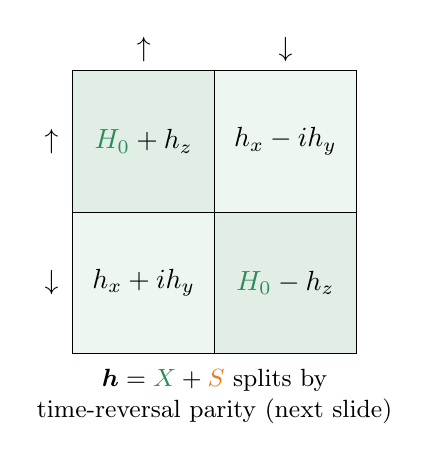
\begin{tikzpicture}[scale=0.9]
\draw[fill=cH!15] (0,0) rectangle (2,2); \node at (1,1) {$\cH{H_0}+h_z$};
\draw[fill=cH!8] (2,0) rectangle (4,2); \node at (3,1) {$h_x-ih_y$};
\draw[fill=cH!8] (0,-2) rectangle (2,0); \node at (1,-1) {$h_x+ih_y$};
\draw[fill=cH!15] (2,-2) rectangle (4,0); \node at (3,-1) {$\cH{H_0}-h_z$};
\node at (1,2.3) {$\uparrow$}; \node at (3,2.3) {$\downarrow$};
\node at (-0.3,1) {$\uparrow$}; \node at (-0.3,-1) {$\downarrow$};
\node[align=center,font=\small] at (2,-2.6) {$\bm h=\X+\SO$ splits by\\ time-reversal parity (next slide)};
\end{tikzpicture}
\end{columns}
\end{frame}

\begin{frame}{Exchange vs.\ spin--orbit: time-reversal split}
\begin{eqbox}[Claim]{cH}
In a time-reversal-symmetric (real) orbital gauge, $\ \X=\operatorname{Re}\bm h$ is \emph{time-odd} (exchange) and $\ \SO=i\operatorname{Im}\bm h$ is \emph{time-even} (SOC).
\end{eqbox}
\begin{proofbox}
$\Theta=i\sigma_y\mathcal K$, $\Theta\sigma_c\Theta^{-1}=-\sigma_c$, and $\mathcal K$ conjugates the orbital matrices (real basis functions):
\[
\Theta\big(M\otimes\sigma_c\big)\Theta^{-1}=-M^{*}\otimes\sigma_c .
\]
Hence the time-even part of $\bm h$ satisfies $M^{*}=-M$ (purely imaginary) and the time-odd part $M^{*}=M$ (real). Hermiticity of $\Hm$ gives $\bm h(\bm R)^\dagger=\bm h(-\bm R)$, so $\operatorname{Re}\bm h$ is symmetric and $i\operatorname{Im}\bm h$ antisymmetric: atomic $\cS{\xi\bm L\cdot\bm S}$ has $\bm L$ imaginary-antisymmetric in a real basis. \qedb
\end{proofbox}
\small\textbf{Diagnostic:} $\max|\operatorname{Im}\cH{H_0}|$ is stored; spinor MLWFs are only approximately real, which is why the code also checks $E(\n)=E(-\n)$ for the MAE.
\end{frame}

\begin{frame}{Assigning Wannier functions to atoms and to the home cell}
\begin{columns}[c]
\column{0.55\textwidth}
\small
\begin{itemize}
\item Atom of each WF from the \texttt{projections} block (robust), checked against \texttt{\_centres.xyz}.
\item A centre close to an \emph{image} $\bm\tau_a+\bm T_m$ is moved home: $w'_m(\bm r)=w_m(\bm r+\bm T_m)$.
\end{itemize}
\begin{eqbox}[Home-cell shift \cC{\_home\_shift}]{cH}
\[
\cH{H'_{mn}(\bm R)}=\cH{H_{mn}}(\bm R+\bm T_n-\bm T_m)
\]
\end{eqbox}
\begin{proofbox}
$\langle w'_{m\bm 0}|\hat H|w'_{n\bm R}\rangle=\langle w_{m,-\bm T_m}|\hat H|w_{n,\bm R-\bm T_n}\rangle$ and translation invariance moves $-\bm T_m$ to the origin. \qedb
\end{proofbox}
\small Residual distance $>$ \texttt{wf\_centre\_tol} (0.6 \AA) stops the run: bond-centred MLWFs cannot be attributed to an atom.
\column{0.42\textwidth}
\centering
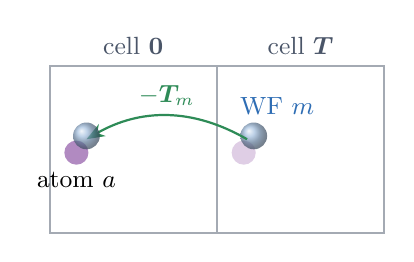
\begin{tikzpicture}[scale=0.85]
\foreach \x in {0,2.5}{\draw[thick,cC!50] (\x,0) rectangle ++(2.5,2.5);}
\node[cC] at (1.25,2.8) {\small cell $\bm 0$}; \node[cC] at (3.75,2.8) {\small cell $\bm T$};
\fill[cR!60] (0.4,1.2) circle (0.18); \node at (0.4,0.8) {\small atom $a$};
\fill[cR!25] (2.9,1.2) circle (0.18);
\shade[ball color=cG!60,opacity=0.7] (3.05,1.45) circle (0.2);
\node[cG] at (3.4,1.9) {\small WF $m$};
\draw[-Stealth,thick,cH] (2.95,1.4) to[bend right=30] node[above,font=\small]{$-\bm T_m$} (0.55,1.4);
\shade[ball color=cG!60,opacity=0.7] (0.55,1.45) circle (0.2);
\end{tikzpicture}
\end{columns}
\end{frame}

\begin{frame}{Atomic spin--orbit coupling on the Wannier orbitals \src{orbitals.py}}
\begin{columns}[c]
\column{0.58\textwidth}
\small
Wannier90 real harmonics: $p:(p_z,p_x,p_y)$, $d:(d_{z^2},d_{xz},d_{yz},d_{x^2-y^2},d_{xy})$, $f$: 7 functions.
\begin{eqbox}[$\bm L$ built from the polynomials themselves]{cS}
\[
\cS{L_\alpha}\, Y_m=-i(\bm r\times\nabla)_\alpha Y_m=\sum_{m'}Y_{m'}\,C^{\alpha}_{m'm}
\]
\end{eqbox}
evaluated on a Gauss--Legendre $\times$ uniform-$\phi$ grid (exact for these polynomials), normalised with exact norms. No tabulated phases $\Rightarrow$ no sign errors.
\begin{eqbox}[Added to the on-site block]{cS}
\[
\cS{\xi_l\,\bm L\cdot\bm S}=\sum_c \underbrace{\tfrac{\xi_l}{2}\cS{L_c}}_{\SO_c}\otimes\sigma_c
\]
\end{eqbox}
Checks: $[L_x,L_y]=iL_z$, $\bm L^2=l(l{+}1)$, eigenvalues of $\bm L\!\cdot\!\bm S$: $\tfrac l2$ and $-\tfrac{l+1}2$.
\column{0.40\textwidth}
\centering
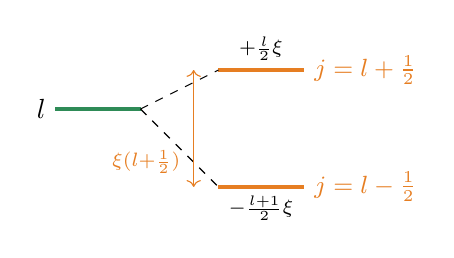
\begin{tikzpicture}[scale=0.9]
\draw[very thick,cH] (0,0) -- (1.2,0); \node[left] at (0,0) {$l$};
\draw[very thick,cS] (2.3,0.55) -- (3.5,0.55) node[right,font=\small]{$j=l+\tfrac12$};
\draw[very thick,cS] (2.3,-1.1) -- (3.5,-1.1) node[right,font=\small]{$j=l-\tfrac12$};
\draw[dashed] (1.2,0) -- (2.3,0.55); \draw[dashed] (1.2,0)--(2.3,-1.1);
\draw[<->,cS] (1.95,0.55)--(1.95,-1.1); \node[cS,left,font=\scriptsize] at (1.9,-0.75) {$\xi(l{+}\tfrac12)$};
\node[font=\scriptsize] at (2.9,0.85) {$+\tfrac{l}{2}\xi$};
\node[font=\scriptsize] at (2.9,-1.4) {$-\tfrac{l+1}{2}\xi$};
\end{tikzpicture}\\[6pt]
\small default $\xi$ table (Cr 35, Fe 55, Pt 600, I 600, Bi 1250 meV); override with \texttt{[soc\_xi]}.
\end{columns}
\end{frame}

\begin{frame}{Rotating the magnetisation relative to the lattice}
\begin{columns}[c]
\column{0.55\textwidth}
\begin{eqbox}[\cC{TBModel.rotated(R)}]{cR}
\[
\X_c(\bm R)\;\longrightarrow\;\sum_{d}\cR{\mathcal R_{cd}}\,\X_d(\bm R),\qquad \cH{H_0},\ \SO\ \text{fixed}
\]
\end{eqbox}
\small
\begin{itemize}
\item rotates the spin direction of the \emph{exchange} field only: the physical rotation of the magnetisation with the crystal and SOC fixed.
\item one collinear DFT run + $\cS{\xi\bm L\!\cdot\!\bm S}$ gives exact model-level references along $x$, $y$, $z$ (or any $\n$).
\item a rotation of the \emph{full} spin space would be a gauge change and leave all energies unchanged.
\end{itemize}
\cC{rotation\_to(n)}: Rodrigues rotation taking $\hat z\to\n$.
\column{0.42\textwidth}
\centering
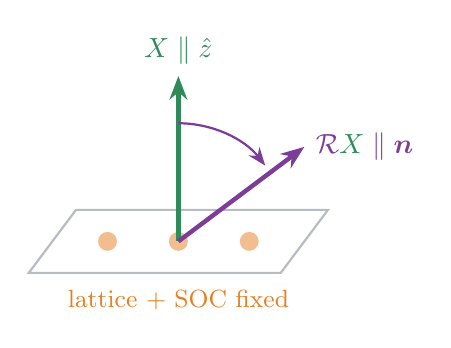
\begin{tikzpicture}[scale=1.0]
\draw[cC!40,thick] (-1.6,-1.2) -- (1.6,-1.2) -- (2.2,-0.4) -- (-1,-0.4) -- cycle;
\foreach \x in {-0.9,0,0.9}{\fill[cS!50] (\x+0.3,-0.8) circle (0.12);}
\node[cS,font=\small] at (0.3,-1.55) {lattice + SOC fixed};
\draw[-{Stealth[length=3mm]},line width=1.6pt,cH] (0.3,-0.8) -- (0.3,1.3) node[above]{$\X\parallel\hat z$};
\draw[-{Stealth[length=3mm]},line width=1.6pt,cR] (0.3,-0.8) -- (1.9,0.4) node[right]{$\cR{\mathcal R}\X\parallel\n$};
\draw[-Stealth,cR,thick] (0.3,0.7) arc (90:38:1.4);
\end{tikzpicture}
\end{columns}
\end{frame}

% =====================================================================
\section{Magnetic force theorem}
% =====================================================================
\begin{frame}{Counting states: the Lloyd formula}
\begin{eqbox}[Integrated density of states]{cE}
\[
N(\varepsilon)=N_{\rm tot}-\frac1\pi\operatorname{Im}\operatorname{Tr}\ln\!\big(\varepsilon+i0^+-\Hm\big)
\]
\end{eqbox}
\begin{proofbox}
For one level $E$: $\ln(\varepsilon+i0-E)=\ln|\varepsilon-E|+i\pi\,\theta(E-\varepsilon)$. Summing over eigenvalues, $\frac1\pi\operatorname{Im}\operatorname{Tr}\ln$ counts the levels \emph{above} $\varepsilon$. \qedb
\end{proofbox}
\begin{eqbox}[Variation under $\Hm\to\Hm+\cK{V}$]{cE}
\[
\delta N(\varepsilon)=-\frac1\pi\operatorname{Im}\operatorname{Tr}\ln(1-\G\cK V)
=\frac1\pi\operatorname{Im}\operatorname{Tr}\Big[\G\cK V+\tfrac12\G\cK V\G\cK V+\dots\Big],\qquad \G=(\varepsilon+i0-\Hm)^{-1}
\]
\end{eqbox}
\small using $\ln(\varepsilon-\Hm-\cK V)-\ln(\varepsilon-\Hm)=\ln\!\big(1-\G\cK V\big)$ inside the trace.
\end{frame}

\begin{frame}{Grand potential and the force theorem}
\begin{eqbox}[Frozen-potential grand potential at fixed $\mus$]{cE}
\[
\Om=-k_BT\sum_{n}\ln\!\big(1+e^{-(\varepsilon_n-\mus)/k_BT}\big)=-\int d\varepsilon\,\fF(\varepsilon)\,N(\varepsilon)
\]
\end{eqbox}
\begin{proofbox}
$\frac{d}{d\varepsilon}\big[-k_BT\ln(1+e^{-(\varepsilon-\mu)/k_BT})\big]=f(\varepsilon)$; integrate $\Om=\int n(\varepsilon)\,(\cdots)\,d\varepsilon$ by parts with $n=dN/d\varepsilon$. \qedb
\end{proofbox}
\begin{eqbox}[Second-order energy change]{cE}
\[
\delta\Om=-\frac1\pi\operatorname{Im}\!\int\! d\varepsilon\,\fF(\varepsilon)\operatorname{Tr}\Big[\G\cK V+\tfrac12\G\cK V\G\cK V\Big]
\]
\end{eqbox}
\small
\textbf{Force theorem:} to second order the self-consistent energy change equals this band (grand-potential) change at frozen potential, because the first-order density response does not change the functional's stationary value. The code computes $\Om$-curvatures \emph{exactly}; the only approximation is the frozen potential.
\end{frame}

\begin{frame}{The perturbation: a rigid rotation of one site's exchange field}
\begin{columns}[c]
\column{0.6\textwidth}
\small Rotation by $\ph$ about axis $\e_a$ in spin space: $U=e^{-i\ph\,\e_a\cdot\sig/2}$.
\begin{eqbox}[First derivative]{cK}
\[
\frac{\partial \Hm}{\partial\ph_{a}}\Big|_0=-\tfrac i2[\sigma_a,\p\!\cdot\!\sig]=(\e_a\times\p)\cdot\sig\equiv\W_a
\]
\end{eqbox}
\begin{proofbox}
$[\sigma_a,\sigma_b]=2i\epsilon_{abc}\sigma_c\Rightarrow -\tfrac i2[\sigma_a,p_b\sigma_b]=\epsilon_{abc}\,p_b\sigma_c=(\e_a\times\p)_c\sigma_c$. \qedb
\end{proofbox}
\begin{eqbox}[Second derivative (symmetrised)]{cK}
\[
\frac{\partial^2\Hm}{\partial\ph_a\partial\ph_b}=\tfrac12\big[\e_a\times(\e_b\times\p)+\e_b\times(\e_a\times\p)\big]\cdot\sig
\]
\end{eqbox}
\column{0.38\textwidth}
\centering
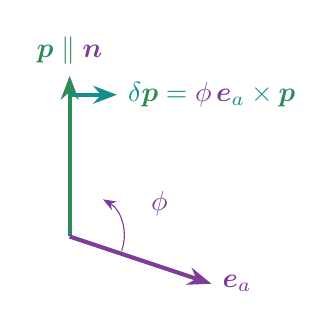
\begin{tikzpicture}[scale=1.2]
\draw[-{Stealth[length=3mm]},line width=1.5pt,cH] (0,0) -- (0,1.7) node[above]{$\p\parallel\n$};
\draw[-{Stealth[length=3mm]},line width=1.5pt,cR] (0,0) -- (1.5,-0.5) node[right]{$\e_a$};
\draw[-{Stealth[length=3mm]},line width=1.5pt,cK] (0,1.5) -- (0.5,1.5) node[right]{$\delta\p=\ph\,\e_a\times\p$};
\draw[cR,-Stealth] (0.55,-0.15) arc (-20:60:0.45);
\node[cR] at (0.95,0.35) {$\ph$};
\end{tikzpicture}\\[4pt]
\small $\p_i$: time-odd on-site field of site $i$ (\cC{onsite\_exchange}). Only $\e_a\perp\n$ gives a non-zero $\W_a$.
\end{columns}
\end{frame}

\begin{frame}{The energy Hessian}
\begin{eqbox}[Two-site and on-site Hessians \src{engine.py}]{cK}
\[
\K_{ab}(i,j,\bm R)\equiv\frac{\partial^2\Om}{\partial\ph_{ia}\partial\ph_{jb}}
=-\frac1\pi\operatorname{Im}\!\int\!d\varepsilon\,\fF(\varepsilon)\operatorname{Tr}\big[\W_{ia}\,\G_{ij}(\bm R)\,\W_{jb}\,\G_{ji}(-\bm R)\big]
\]
\[
\frac{\partial^2\Om}{\partial\ph_{ia}\partial\ph_{ib}}=\tfrac12\big[\K_{ab}(i,i,\bm 0)+\K_{ba}(i,i,\bm 0)\big]+\T_{ab}(i),\qquad
\T_{ab}(i)=\operatorname{Tr}\!\Big[\rho_{ii}\,\frac{\partial^2\Hm_i}{\partial\ph_a\partial\ph_b}\Big]
\]
\end{eqbox}
\begin{proofbox}[Why the cross term has no factor $\tfrac12$]
With $\cK V=\ph_{ia}\W_{ia}+\ph_{jb}\W_{jb}$, the term $\tfrac12\operatorname{Tr}[\G\cK V\G\cK V]$ contains $\ph_{ia}\ph_{jb}\operatorname{Tr}[\G\W_{ia}\G\W_{jb}]$ twice $\times\tfrac12$ (cyclicity). The first-order term with $\partial^2\Hm$ gives $\T$ via $\rho=-\frac1\pi\operatorname{Im}\int f\,\G$. \qedb
\end{proofbox}
\small $\G_{ij}(\bm R)$: block between site $i$ in cell $\bm 0$ and site $j$ in cell $\bm R$. All 9 axis pairs $(a,b)$ are computed; those with $\e\parallel\n$ vanish.
\end{frame}

\begin{frame}{Green's functions in practice}
\begin{columns}[c]
\column{0.57\textwidth}
\begin{eqbox}[Spectral form (no matrix inversion per $z$)]{cG}
\[
\G(\bm k,z)=\Psim_{\bm k}\,\mathrm{diag}\Big(\frac{1}{z-\cG{\varepsilon_{n\bm k}}}\Big)\Psim_{\bm k}^\dagger
\]
\end{eqbox}
\begin{eqbox}[To real space by FFT]{cG}
\[
\G(\bm R,z)=\frac1{N_k}\sum_{\bm k}\G(\bm k,z)\,e^{-2\pi i\bm k\cdot\bm R}=\texttt{fftn}/N_k
\]
\[
\G(-\bm R)=\texttt{roll(flip}(\G),1)
\]
\end{eqbox}
\small
\begin{itemize}
\item only rows/columns of the spin sites are kept: $\Psim_{\rm sel}$ of shape $(N_k,N_{\rm sel},N_b)$
\item $\Gamma$-centred mesh $\Rightarrow$ $\bm R$ lives on the $N_1\!\times\!N_2\!\times\!N_3$ supercell
\item test: $\K$ from the $k$-mesh $=$ $\Gamma$-only explicit supercell to $9\times10^{-16}$
\end{itemize}
\column{0.40\textwidth}
\centering
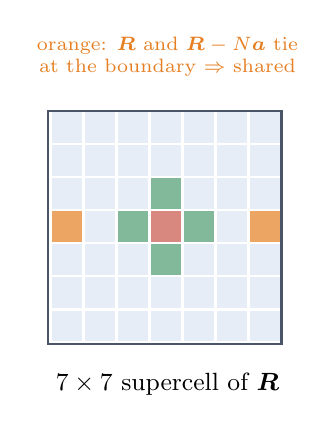
\begin{tikzpicture}[scale=0.42]
\foreach \x in {0,...,6}{\foreach \y in {0,...,6}{
  \fill[cG!12] (\x,\y) rectangle ++(0.92,0.92);}}
\fill[cJ!60] (3,3) rectangle ++(0.92,0.92);
\foreach \p in {(4,3),(2,3),(3,4),(3,2)}{\fill[cH!60] \p rectangle ++(0.92,0.92);}
\fill[cS!70] (6,3) rectangle ++(0.92,0.92); \fill[cS!70] (0,3) rectangle ++(0.92,0.92);
\draw[thick,cC] (-0.1,-0.1) rectangle (6.95,6.95);
\node[font=\small,align=center] at (3.5,-1.3) {$7\times7$ supercell of $\bm R$};
\node[font=\scriptsize,cS,align=center] at (3.5,8.6) {orange: $\bm R$ and $\bm R-N\bm a$ tie\\at the boundary $\Rightarrow$ shared};
\end{tikzpicture}
\end{columns}
\end{frame}

% =====================================================================
\section{Energy integration}
% =====================================================================
\begin{frame}{Fermi--Dirac via Ozaki poles \src{contour.py}}
\begin{columns}[T]
\column{0.5\textwidth}
\begin{eqbox}[Continued-fraction expansion]{cE}
\[
\fF(x)=\tfrac12-\sum_{p=1}^{N_p}\cE{R_p}\Big[\tfrac{1}{x-i\cE{z_p}}+\tfrac{1}{x+i\cE{z_p}}\Big]
\]
\end{eqbox}
\small $\cE{z_p}=1/\lambda_p$ from the eigenvalues $\lambda_p>0$ of the tridiagonal $B$, $b_n=\tfrac{1}{2\sqrt{(2n-1)(2n+1)}}$; $\cE{R_p}=|v_{1p}|^2/4\lambda_p^2$.
\begin{eqbox}[Contour result]{cE}
\[
-\frac1\pi\operatorname{Im}\!\int\fF\,F(\varepsilon^+)\,d\varepsilon=2k_BT\sum_p \cE{R_p}\operatorname{Re}F(\mus+i\cE{z_p}k_BT)
\]
\end{eqbox}
\column{0.48\textwidth}
\begin{proofbox}
$F$ analytic in the UHP and $F\sim z^{-2}$: close the real line in the UHP. $\int F/2=0$; only the poles of $\fF$ at $\mus+iz_pk_BT$ (residue $-R_pk_BT$) contribute:
$\int fF=-2\pi i\,k_BT\sum_pR_pF(z_p)$. Take $-\frac1\pi\operatorname{Im}$. \qedb
\end{proofbox}
\small\textbf{Why $F\sim z^{-2}$:} every perturbation is a Pauli matrix, $\operatorname{Tr}_\sigma\sigma_c=0$, so the $1/z$ term $\operatorname{Tr}\cK V/z$ vanishes.\\[3pt]
\textbf{Gain:} no $E_{\min}$, 60 poles for 30 eV at 300 K, $\mus+i\pi k_BT$ smooths $k$-sums in metals.
\end{columns}
\end{frame}

\begin{frame}{Integration nodes and convergence}
\centering
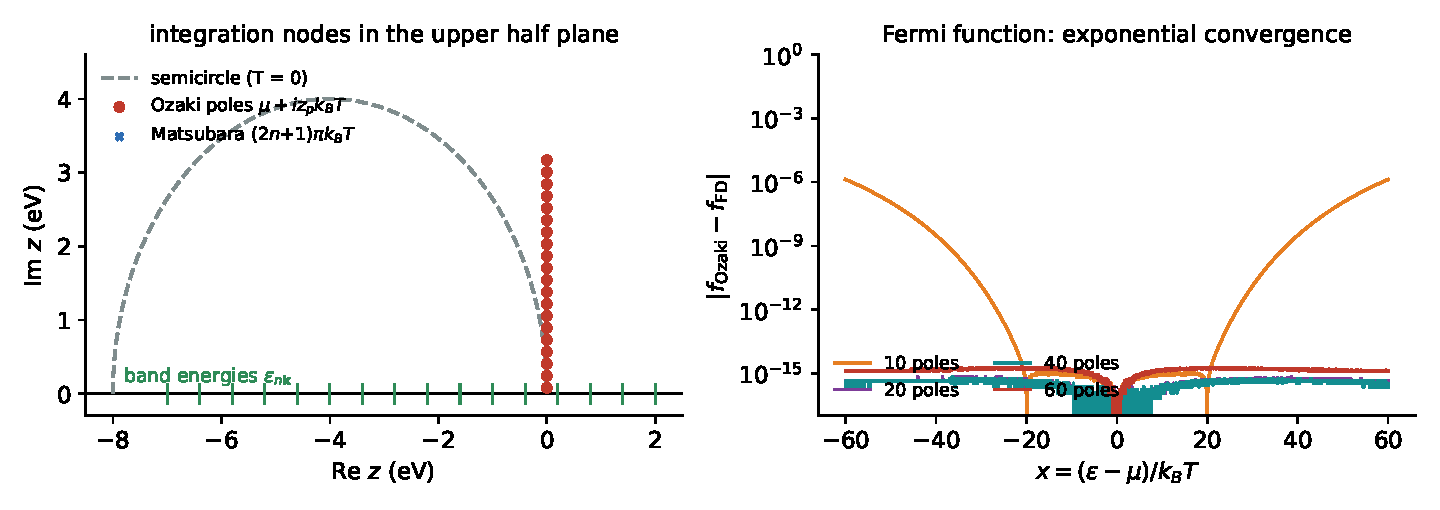
\includegraphics[width=0.98\textwidth]{figs/contour.pdf}\\[2pt]
\small Left: Ozaki poles sit on the line $\operatorname{Re}z=\mus$, sparser than Matsubara frequencies and far from all bands. Right: error of the Fermi function vs.\ number of poles; \cC{ozaki\_npoles} picks the smallest $N_p$ reaching $10^{-10}$ over the band width. The $T=0$ semicircle (Gauss--Legendre in angle) is kept as an option.
\end{frame}

% =====================================================================
\section{Rotational invariance}
% =====================================================================
\begin{frame}{The Goldstone sum rule}
\begin{eqbox}[Exact statement (no SOC)]{cK}
A uniform rotation of \emph{all} spins is a symmetry $\Rightarrow$ $\Om$ is constant along it:
\[
\sum_{j,\bm R}\K_{aa}(i,j,\bm R)+\T_{aa}(i)=0\qquad\forall\,i
\]
\end{eqbox}
\begin{proofbox}
Rotate every site by the same $\ph$: $\Om(\ph)-\Om(0)=\tfrac12\ph^2\sum_{ij\bm R}\partial^2\Om=0$ only if the rotated operators add up to the generator of a \emph{global} rotation, $\sum_i\delta\Hm_i=(\e_a\times\X)\cdot\sig$ for the full $\X(\bm R)$. \qedb
\end{proofbox}
\begin{columns}[c]
\column{0.5\textwidth}
\small LKAG/TB2J rotate only $\p_i=\X_{ii}(\bm 0)$. In Wannier bases the exchange field also lives on inter-atomic elements $\X_{ij}(\bm R)$, which then never rotate.
\column{0.48\textwidth}
\centering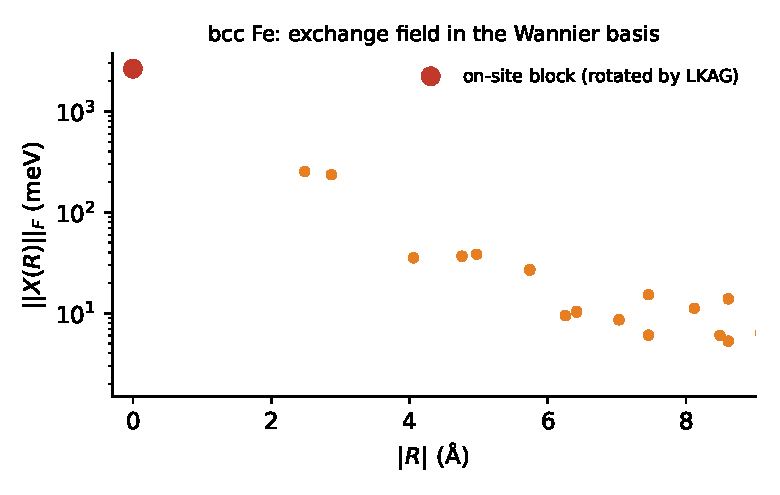
\includegraphics[height=3.6cm]{figs/fe_X_decay.pdf}
\end{columns}
\end{frame}

\begin{frame}{Partitioning the exchange field among atoms \src{engine\_partition.py}}
\begin{columns}[c]
\column{0.58\textwidth}
\begin{eqbox}[Weighted partition]{cH}
\[
\X=\sum_i\X^{(i)},\qquad \X^{(i)}=\Pi_i\X_L+\X_L^\dagger\Pi_i
\]
\[
(\X_L)_{mn}(\bm R)=f_{a(m)a(n)}\,\X_{mn}(\bm R),\quad f_{ab}=\frac{w_a}{w_a+w_b}
\]
\end{eqbox}
\small $w_a=\|\p_a\|$; $f_{aa}=\tfrac12$. $\Pi_i$ projects on the orbitals of atom $i$ in cell $\bm 0$.
\begin{proofbox}[$\sum_i\X^{(i)}=\X$]
$\sum_i\Pi_i=1$ over all atoms and cells, so $\sum_i\X^{(i)}=\X_L+\X_L^\dagger$. Element-wise $(\X_L+\X_L^\dagger)_{mn}=(f_{ab}+f_{ba})\X_{mn}=\X_{mn}$ using $\X^\dagger=\X$. \qedb
\end{proofbox}
\column{0.40\textwidth}
\centering
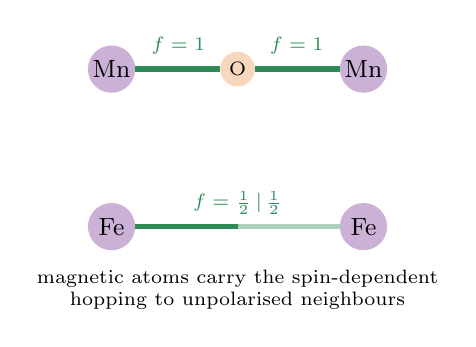
\begin{tikzpicture}[scale=1.0]
\fill[cR!40] (0,0) circle (0.3) node[text=black]{\small Mn}; \fill[cR!40] (3.2,0) circle (0.3) node[text=black]{\small Mn};
\fill[cS!30] (1.6,0) circle (0.22) node[text=black]{\scriptsize O};
\draw[cH,line width=2pt] (0.3,0) -- (1.38,0); \draw[cH,line width=2pt] (1.82,0)--(2.9,0);
\node[cH,font=\scriptsize] at (0.85,0.3) {$f=1$}; \node[cH,font=\scriptsize] at (2.35,0.3) {$f=1$};
\fill[cR!40] (0,-2) circle (0.3) node[text=black]{\small Fe}; \fill[cR!40] (3.2,-2) circle (0.3) node[text=black]{\small Fe};
\draw[cH,line width=2pt] (0.3,-2) -- (1.6,-2); \draw[cH!40,line width=2pt] (1.6,-2)--(2.9,-2);
\node[cH,font=\scriptsize] at (1.6,-1.7) {$f=\tfrac12\,|\,\tfrac12$};
\node[font=\scriptsize,align=center] at (1.6,-2.8) {magnetic atoms carry the spin-dependent\\hopping to unpolarised neighbours};
\end{tikzpicture}
\end{columns}
\takeaway{rotating every $\X^{(i)}$ by the same angle is an exact global spin rotation, so the sum rule holds identically.}
\end{frame}

\begin{frame}{Non-local perturbation: four-term trace}
\begin{eqbox}[Perturbation of site $i$]{cK}
\[
\W_{ia}=\Pi_i\cH{Y_a}+\cH{Y_a}^\dagger\Pi_i,\qquad \cH{Y_a}=(\e_a\times\X_L)\cdot\sig
\]
\end{eqbox}
\begin{eqbox}[Trace (\cC{engine\_partition})]{cK}
\[
\begin{aligned}
\operatorname{Tr}[\W_{ia}\G\W_{jb}\G]=\ &\operatorname{Tr}\big[(\cH{Y_a}\G)_{ij}(\cH{Y_b}\G)_{ji}\big]+\operatorname{Tr}\big[(\cH{Y_a}\G\cH{Y_b}^\dagger)_{ij}\G_{ji}\big]\\
+\ &\operatorname{Tr}\big[\G_{ij}(\cH{Y_b}\G\cH{Y_a}^\dagger)_{ji}\big]+\operatorname{Tr}\big[(\G\cH{Y_b}^\dagger)_{ij}(\G\cH{Y_a}^\dagger)_{ji}\big]
\end{aligned}
\]
\end{eqbox}
\begin{proofbox}
Expand the product of two sums; move each $\Pi$ by cyclicity, e.g. $\operatorname{Tr}[\cH{Y_a}^\dagger\Pi_i\G\cH{Y_b}^\dagger\Pi_j\G]=\operatorname{Tr}[\Pi_i(\G\cH{Y_b}^\dagger)\Pi_j(\G\cH{Y_a}^\dagger)]$; $\Pi_i\cdots\Pi_j$ selects the $(i,j)$ block. \qedb
\end{proofbox}
\small The on-site first-order term becomes $\T_{ab}(i)=\operatorname{Tr}_i[(\cH{Z_{ab}}\rho)_{ii}+(\rho\cH{Z_{ab}}^\dagger)_{ii}]$, $\cH{Z_{ab}}=\tfrac12[\e_a\times(\e_b\times\X_L)+(a\leftrightarrow b)]\cdot\sig$.
\end{frame}

\begin{frame}{Evaluating the four terms efficiently}
\begin{columns}[c]
\column{0.55\textwidth}
\small Precompute once per $\bm k$ (independent of $z$):
\[
\cG{U_a(\bm k)}=\cH{Y_a(\bm k)}[\text{sel},:]\,\Psim_{\bm k},\qquad \cG{Q_{ab}(\bm k)}=\cH{Z_{ab}(\bm k)}[\text{sel},:]\,\Psim_{\bm k}
\]
Then every block has the form $A\,\mathrm{diag}(g)\,B^\dagger$ with $g_n=1/(z-\cG{\varepsilon_{n\bm k}})$:
\[
\begin{aligned}
\G&=\Psim_{\rm s}g\Psim_{\rm s}^\dagger, & \cH Y_a\G&=\cG{U_a}g\Psim_{\rm s}^\dagger,\\
\G\cH Y_b^\dagger&=\Psim_{\rm s}g\cG{U_b}^\dagger, & \cH Y_a\G\cH Y_b^\dagger&=\cG{U_a}g\cG{U_b}^\dagger
\end{aligned}
\]
16 batched \texttt{matmul}s + 16 FFTs per energy node.
\column{0.42\textwidth}
\begin{plainbox}{cC}
\small\textbf{Exact checks}
\begin{itemize}
\item \texttt{partition="onsite"} reproduces the fast engine to $4\times10^{-16}$
\item weighted Hessian vs.\ finite differences of the partitioned rotation: $1.3\times10^{-7}$
\item sum rule: $4\times10^{-15}$
\end{itemize}
\end{plainbox}
\vspace{2pt}
\centering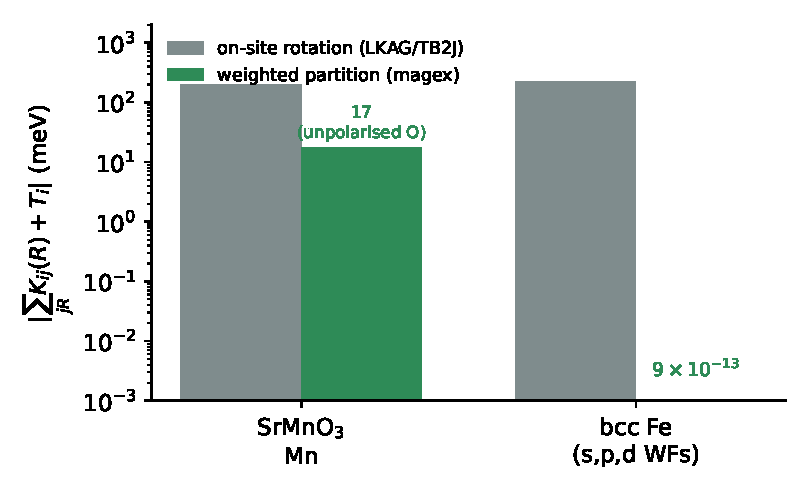
\includegraphics[height=3.4cm]{figs/sumrule.pdf}
\end{columns}
\end{frame}

% =====================================================================
\section{From Hessians to spin-model parameters}
% =====================================================================
\begin{frame}{Heisenberg Hessian}
\begin{eqbox}[Mapping used for every pair \src{heisenberg.py}]{cJ}
\[
\K_{ab}(i,j,\bm R)=-2\,(\e_a\times\n_i)\cdot\J_{ij}(\bm R)\cdot(\e_b\times\n_j)
\]
\end{eqbox}
\begin{proofbox}
Rotating $\e_i=\cR{\mathcal R}(\ph_i)\n_i$ gives $\delta\e_i=\ph_{ia}\,\e_a\times\n_i+O(\ph^2)$. The pair $(i,j)$ enters $E$ as $-\e_i\!\cdot\!\J_{ij}\!\cdot\!\e_j-\e_j\!\cdot\!\J_{ji}\!\cdot\!\e_i=-2\,\e_i\!\cdot\!\J_{ij}\!\cdot\!\e_j$, whose mixed derivative is $-2(\e_a\times\n_i)\!\cdot\!\J_{ij}\!\cdot\!(\e_b\times\n_j)$. Second-order terms in $\delta\e_i$ multiply $\n_j$ and do not contribute to $\partial_{\ph_i}\partial_{\ph_j}$. \qedb
\end{proofbox}
\small
\begin{itemize}
\item collinear reference: $\n_i=s_i\hat{\bm d}$ with $s_i=\operatorname{sign}(\bm M_i\cdot\hat{\bm d})$ (AFM handled automatically)
\item isotropic, no SOC: $\K_{aa}=-2s_is_j\,\cJ{J_{ij}}$ for $a\perp\hat{\bm d}$; equivalent to LKAG $\cJ{J}=\tfrac1{4\pi}\operatorname{Im}\!\int\!\operatorname{Tr}[\Delta_i\G^\uparrow_{ij}\Delta_j\G^\downarrow_{ji}]$ averaged over $i\!\leftrightarrow\!j$
\end{itemize}
\end{frame}

\begin{frame}{Three references from one Hamiltonian}
\begin{columns}[c]
\column{0.5\textwidth}
\small Each reference $\hat{\bm d}$ gives 4 equations (axes $\perp\hat{\bm d}$):
\begin{itemize}
\item $\hat{\bm d}=\hat z$: $J_{xx},J_{xy},J_{yx},J_{yy}$
\item $\hat{\bm d}=\hat x$: $J_{yy},J_{yz},J_{zy},J_{zz}$
\item $\hat{\bm d}=\hat y$: $J_{zz},J_{zx},J_{xz},J_{xx}$
\end{itemize}
12 equations, 9 unknowns $\Rightarrow$ least squares:
\begin{eqbox}[Joint fit]{cJ}
\[
\min_{\J_{ij}}\sum_{\hat{\bm d}}\sum_{a,b}\Big|\K^{(\hat{\bm d})}_{ab}+2(\e_a\!\times\!\n_i)\!\cdot\!\J_{ij}\!\cdot\!(\e_b\!\times\!\n_j)\Big|^2
\]
\end{eqbox}
residual $=$ \textbf{reference dependence} (printed per pair).
\column{0.47\textwidth}
\centering
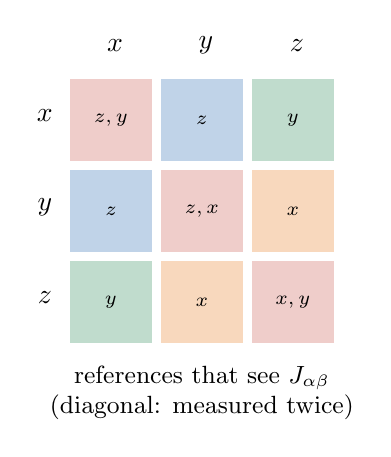
\begin{tikzpicture}[scale=1.05]
\foreach \i/\r in {0/x,1/y,2/z}{\node at (\i*1.1+0.55,3.6) {$\r$}; \node at (-0.3,2.75-\i*1.1) {$\r$};}
\cellfill{0}{0}{cJ!25}\cellfill{1}{0}{cG!30}\cellfill{2}{0}{cH!30}
\cellfill{0}{1}{cG!30}\cellfill{1}{1}{cJ!25}\cellfill{2}{1}{cS!30}
\cellfill{0}{2}{cH!30}\cellfill{1}{2}{cS!30}\cellfill{2}{2}{cJ!25}
\node[font=\scriptsize,align=center] at (0.5,2.7) {$z,y$}; \node[font=\scriptsize] at (1.6,2.7) {$z$}; \node[font=\scriptsize] at (2.7,2.7) {$y$};
\node[font=\scriptsize] at (0.5,1.6) {$z$}; \node[font=\scriptsize] at (1.6,1.6) {$z,x$}; \node[font=\scriptsize] at (2.7,1.6) {$x$};
\node[font=\scriptsize] at (0.5,0.5) {$y$}; \node[font=\scriptsize] at (1.6,0.5) {$x$}; \node[font=\scriptsize] at (2.7,0.5) {$x,y$};
\node[font=\small,align=center] at (1.6,-0.6) {references that see $J_{\alpha\beta}$\\(diagonal: measured twice)};
\end{tikzpicture}
\end{columns}
\takeaway{one collinear DFT run $+$ $\cS{\xi\bm L\!\cdot\!\bm S}$ $\to$ $\J^{\rm iso}$, $\J^{\rm ani}$ and $\Dv$ for all pairs; no three-run merge, no inter-run Wannier noise.}
\end{frame}

\begin{frame}{Single-ion anisotropy from the on-site Hessian}
\begin{eqbox}[Energy of site $i$ alone rotated (all other spins frozen)]{cJ}
\[
E_i(\e)=\e\cdot\A_i\cdot\e+\bm c\cdot\e,\qquad \bm c=-2\!\!\sum_{(j,\bm R)\neq(i,\bm 0)}\!\!\J_{ij}(\bm R)\,\n_j
\]
\end{eqbox}
\begin{eqbox}[Its Hessian (\cC{build\_results})]{cJ}
\[
\frac{\partial^2E_i}{\partial\ph_a\partial\ph_b}=2(\e_a\!\times\!\n)\cdot\A_i\cdot(\e_b\!\times\!\n)+2\,\n\cdot\A_i\cdot\bm S_{ab}+\bm c\cdot\bm S_{ab}+\cK{\delta_i}\,(\e_a\!\times\!\n)\!\cdot\!(\e_b\!\times\!\n)
\]
\[
\bm S_{ab}=\tfrac12\big[\e_a\times(\e_b\times\n)+\e_b\times(\e_a\times\n)\big]
\]
\end{eqbox}
\small
\begin{itemize}
\item equated to $\tfrac12(\K_{ab}+\K_{ba})(i,i,\bm 0)+\T_{ab}(i)$ for all three references; unknowns: 5 components of traceless $\A_i$ and an isotropic offset $\cK{\delta_i}$
\item images of $i$ in other cells are \emph{different} (frozen) sites: they enter linearly through $\bm c$
\item $\cK{\delta_i}$ absorbs any sum-rule violation; without SOC $\A_i=0$ follows automatically
\end{itemize}
\end{frame}

\begin{frame}{Magnetocrystalline anisotropy and its cross-check}
\begin{columns}[c]
\column{0.5\textwidth}
\begin{eqbox}[Band MAE (\cC{grand\_potential\_directions})]{cE}
\[
\Om(\n)=-\frac{k_BT}{N_k}\sum_{n\bm k}\ln\!\Big(1+e^{-(\varepsilon_{n\bm k}(\n)-\mus)/k_BT}\Big)
\]
\end{eqbox}
\small 8 directions and their negatives, dense \texttt{mae\_kmesh}.
\begin{itemize}
\item \textbf{time-reversal check:} $\max|\Om(\n)-\Om(-\n)|/2$ must vanish
\item even part fitted to $\n\cdot\A_{\rm band}\cdot\n$
\item compared with the Heisenberg prediction
\end{itemize}
\[
E_H(\n)=\sum_i\n\!\cdot\!\A_i\!\cdot\!\n-\sum_{ij\bm R}s_is_j\,\n\!\cdot\!\J_{ij}\!\cdot\!\n
\]
\column{0.48\textwidth}
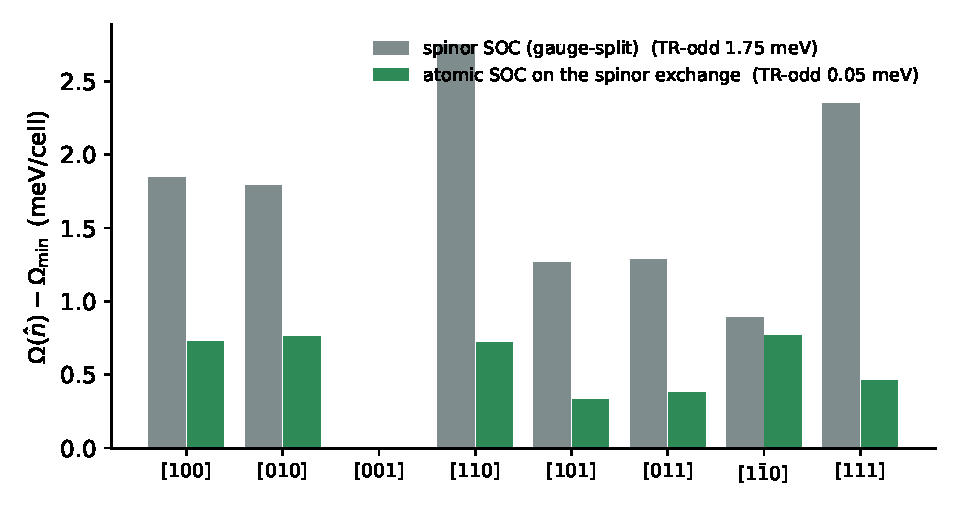
\includegraphics[width=\textwidth]{figs/cri3_mae.pdf}\\
\small CrI$_3$: with gauge-split spinor SOC the TR-odd error is 1.75 meV; with atomic SOC 0.05 meV, easy axis $z$, $K_{\rm eff}=0.71$ (band) vs.\ 0.78 meV/cell (Heisenberg).
\end{columns}
\end{frame}

\begin{frame}{Symmetrisation and supercell aliasing \src{symmetry.py}}
\begin{columns}[T]
\column{0.55\textwidth}
\begin{eqbox}[Group average over the space group (spglib)]{cJ}
\[
\J(p)=\frac1{|\mathcal G|}\sum_{g\in\mathcal G}\cR{\mathcal R_g}^{T}\,\J(g\,p)\,\cR{\mathcal R_g},\qquad \A_i\ \text{likewise}
\]
\end{eqbox}
\begin{proofbox}
$\J$ couples two axial vectors: $\e\to\det(\mathcal R)\mathcal R\e$ for both, $\det^2=1$, so $\J(gp)=\mathcal R\J(p)\mathcal R^T$; time reversal flips both spins and leaves $\J$ unchanged. \qedb
\end{proofbox}
\small Atoms are typed by species and $|\bm M|$; pairs are looked up by their FFT index $\nu=\bm R\bmod N$; the size of the change is printed as the Wannier-noise estimate.
\column{0.42\textwidth}
\small\textbf{Minimal images.} $\bm R\equiv\nu\pmod N$ chosen to minimise $|\bm\tau_j+\bm R-\bm\tau_i|$ (\cC{min\_image}).
At the supercell boundary several images tie: the coupling is \emph{shared}, $\J/n_{\rm img}$ on each (\cC{all\_images}), keeping $\cM{h(\bm k)}$ Hermitian.\\[4pt]
\begin{plainbox}{cS}
\small SrMnO$_3$: before sharing, $h(\bm k)$ was non-Hermitian and LSWT reported a spurious instability.
\end{plainbox}
\end{columns}
\end{frame}

% =====================================================================
\section{Beyond the plain force theorem}
% =====================================================================
\begin{frame}{Bruno renormalisation: rotating moments, not fields}
\begin{columns}[c]
\column{0.6\textwidth}
\small Let $\cR{\theta_i}$ be moment angles and $\ph_i$ field angles; linear response $\theta=\cK{X}\ph$.
\[
\K=\cK{K_b}+\cK D,\qquad \cK{D_i}=\T_i,\qquad \cK{K_b}:\ \text{bubble incl.\ on-site}
\]
\begin{proofbox}[Derivation of $\tilde\K=-\cK D\cK{K_b}^{-1}\cK D-\cK D$]
Hellmann--Feynman: $\partial\Om/\partial\ph=\cK D(\ph-\theta)$, hence $\K=\cK D(1-\cK X)$, $\cK X=-\cK D^{-1}\cK{K_b}$. A constraining field fixes the moments at $\theta$ while the exchange field follows them; total field $\ph_{\rm tot}=\cK X^{-1}\theta$. The constraining torque is $\partial E/\partial\theta=\cK D(\ph_{\rm tot}-\theta)=\cK D(\cK X^{-1}-1)\theta$, so $\tilde\K=\cK D(\cK X^{-1}-1)=-\cK D\cK{K_b}^{-1}\cK D-\cK D$. \qedb
\end{proofbox}
\column{0.38\textwidth}
\begin{eqbox}[One FM sublattice]{cM}
\[
\cM{\tilde\omega(\bm q)}=\frac{\cM{\omega(\bm q)}}{1-\cM{\omega(\bm q)}/\Delta}
\]
\end{eqbox}
\small $\tilde\K=\K+\K\cK D^{-1}\K+\dots$ raises spin-wave energies comparable to the exchange splitting $\Delta$.\\[3pt]
Implemented per $\bm q$ in the magnetic subspace (\cC{renorm.py}); $\cK D$ from the sum rule so that $\tilde\K(\bm 0)$ keeps the Goldstone zero mode.
\end{columns}
\end{frame}

\begin{frame}{Ligand downfolding}
\begin{columns}[c]
\column{0.55\textwidth}
\small Include spin-polarised ligands (O, I, Se \dots) as rotatable sites, then let them relax:
\begin{eqbox}[Schur complement per $\bm q$]{cK}
\[
\K_{\rm eff}(\bm q)=\K_{MM}-\K_{ML}\K_{LL}^{-1}\K_{LM}
\]
\end{eqbox}
\begin{proofbox}
$E=\tfrac12\ph_M^\dagger\K_{MM}\ph_M+\operatorname{Re}\ph_M^\dagger\K_{ML}\ph_L+\tfrac12\ph_L^\dagger\K_{LL}\ph_L$; $\partial E/\partial\ph_L^*=0$ gives $\ph_L=-\K_{LL}^{-1}\K_{LM}\ph_M$; substitute. \qedb
\end{proofbox}
\[
\cJ{J^{\rm DF}_{ij}(\bm R)}=-\frac{1}{2s_is_j}\,\mathrm{FFT}^{-1}\big[\K_{\rm eff}(\bm q)\big]_{ij}
\]
Ligands with $\|\p\|<5$ meV are dropped automatically.
\column{0.42\textwidth}
\centering
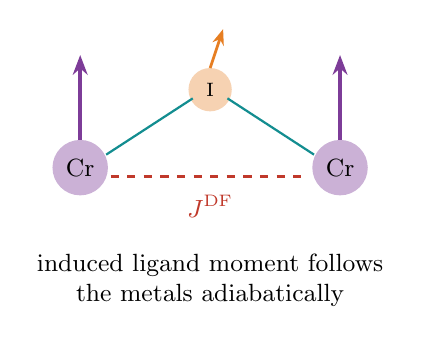
\begin{tikzpicture}[scale=1.1]
\fill[cR!40] (0,0) circle (0.32) node[text=black]{\small Cr}; \fill[cR!40] (3,0) circle (0.32) node[text=black]{\small Cr};
\fill[cS!35] (1.5,0.9) circle (0.25) node[text=black]{\scriptsize I};
\draw[-{Stealth[length=2.5mm]},line width=1.4pt,cR] (0,0.32) -- (0,1.3);
\draw[-{Stealth[length=2.5mm]},line width=1.4pt,cR] (3,0.32) -- (3,1.3);
\draw[-{Stealth[length=2mm]},line width=1pt,cS] (1.5,1.15) -- (1.65,1.6);
\draw[cK,thick] (0.3,0.15) -- (1.3,0.8); \draw[cK,thick] (1.7,0.8) -- (2.7,0.15);
\draw[cJ,very thick,dashed] (0.35,-0.1) -- (2.65,-0.1);
\node[cJ,font=\small] at (1.5,-0.45) {$\cJ{J^{\rm DF}}$};
\node[font=\small,align=center] at (1.5,-1.3) {induced ligand moment follows\\ the metals adiabatically};
\end{tikzpicture}
\end{columns}
\end{frame}

\begin{frame}{Finite angles: exact Lloyd energies}
\begin{eqbox}[Local perturbation of a site set $S$]{cE}
\[
\Delta\Om_S=\frac1\pi\operatorname{Im}\!\int\!d\varepsilon\,\fF\,\ln\det\big(1-\G_{SS}\cK{V}_{SS}\big)
\;=\;-2k_BT\sum_p\cE{R_p}\,\ln\big|\det(1-\G\cK V)\big|_{z_p}
\]
\end{eqbox}
\small $\cK V=(\cR{\mathcal R}(\theta)\X^{(i)}-\X^{(i)})\cdot\sig$, finite. Only $\ln|\det|$ is needed (Ozaki weights are real): no branch cuts.
\begin{proofbox}[Non-local $\cK V$ (weighted partition): Sylvester]
$\cK V=\Pi_i\cH A+\cH A^\dagger\Pi_i=LM$, $L=[\Pi_i\ \cH A^\dagger]$, $M=[\cH A;\Pi_i]$. Then $\det(1-\G LM)=\det(1-M\G L)$, a $2n_i\times 2n_i$ matrix with blocks $(\cH A\G)_{ii}$, $(\cH A\G\cH A^\dagger)_{ii}$, $\G_{ii}$, $(\G\cH A^\dagger)_{ii}$; for a pair, the $4\times4$ block version with phases $e^{\mp2\pi i\bm k\cdot\bm R}$. \qedb
\end{proofbox}
\small Pair interaction energy: $E_{\rm int}=\Delta\Om_{ij}-\Delta\Om_i-\Delta\Om_j$. Exact vs.\ brute-force $\Om$: $2.5\times10^{-11}$ eV.
\end{frame}

\begin{frame}{Bilinear and biquadratic parts of the pair energy}
\begin{columns}[c]
\column{0.55\textwidth}
\small Rotate $i$ by $-\theta/2$ and $j$ by $+\theta/2$; $c=\cos(\theta/2)$, $s=s_is_j$.
\begin{eqbox}[{Model $E=-\sum_{i\neq j}\big[\cJ{J'}\e_i\!\cdot\!\e_j+\cJ B(\e_i\!\cdot\!\e_j)^2\big]$}]{cJ}
\[
E_{\rm int}(\theta)=4s\,\cJ{J'}\,c(1-c)-2\cJ B\cos\theta(\cos\theta-1)
\]
\[
\cJ{J_{\rm small}}=\cJ{J'}+2s\,\cJ B
\]
\end{eqbox}
\begin{proofbox}
$E_{\rm int}=-2J'(\e_i-\n_i)\!\cdot\!(\e_j-\n_j)+\dots$; with $\e_i-\n_i=(-\sin\tfrac\theta2,0,c-1)$, $\e_j-\n_j=s(\sin\tfrac\theta2,0,c-1)$ the dot product is $-2sc(1-c)$. The $B$ term: $(\cos^2\theta-2c^2+1)=\cos\theta(\cos\theta-1)$. Small $\theta$: $E\simeq\tfrac{\theta^2}{2}(sJ'+2B)$. \qedb
\end{proofbox}
\column{0.42\textwidth}
\centering
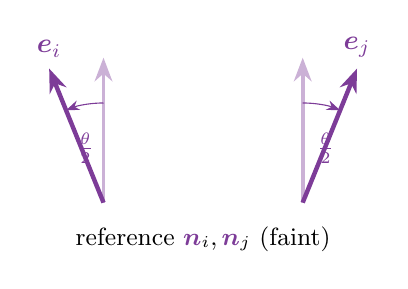
\begin{tikzpicture}[scale=1.15]
\draw[-{Stealth[length=3mm]},line width=1.3pt,cR!40] (0,0) -- (0,1.6);
\draw[-{Stealth[length=3mm]},line width=1.6pt,cR] (0,0) -- (-0.6,1.48) node[above]{$\e_i$};
\draw[-{Stealth[length=3mm]},line width=1.3pt,cR!40] (2.2,0) -- (2.2,1.6);
\draw[-{Stealth[length=3mm]},line width=1.6pt,cR] (2.2,0) -- (2.8,1.48) node[above]{$\e_j$};
\draw[cR,-Stealth] (0,1.1) arc (90:112:1.1); \node[cR,font=\small] at (-0.2,0.6) {$\tfrac\theta2$};
\draw[cR,-Stealth] (2.2,1.1) arc (90:68:1.1); \node[cR,font=\small] at (2.45,0.6) {$\tfrac\theta2$};
\node[font=\small] at (1.1,-0.4) {reference $\n_i,\n_j$ (faint)};
\end{tikzpicture}
\end{columns}
\small The code also draws the \emph{tensor} bilinear curve $-2(\e_i-\n_i)\!\cdot\!\J_{ij}\!\cdot\!(\e_j-\n_j)$ and reports $\max|E_{\rm Lloyd}-E_{\rm bil}|$ as the Heisenberg error.
\end{frame}

\begin{frame}{Lloyd results: how Heisenberg-like are the bonds?}
\centering
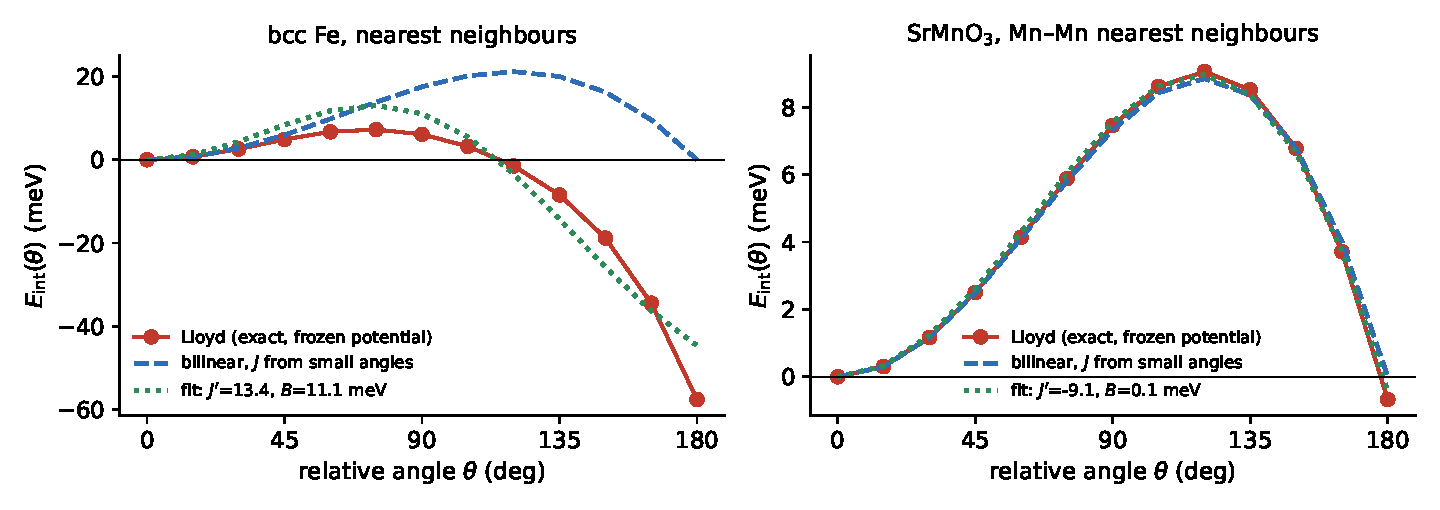
\includegraphics[width=0.97\textwidth]{figs/lloyd.pdf}\\[2pt]
\small SrMnO$_3$ (localised Mn$^{4+}$): the bilinear curve from small angles reproduces the exact pair energy over the full range. bcc Fe: strongly angle-dependent nearest-neighbour coupling, a large effective biquadratic term, in line with Szilva \emph{et al.}, PRL 111, 127204 (2013). Small-angle $\J$ remain the right input for low-temperature magnons.
\end{frame}

% =====================================================================
\section{Spin waves}
% =====================================================================
\begin{frame}{Linear spin-wave theory \src{magnon.py}}
\small Local frames: $\n_i$ (local $z$), $\bm u_i=\bm x_i+i\bm y_i$; spins $S_i=|\bm M_i|/2$; $\tilde\J_{ij}=-\J_{ij}/S_iS_j$, $\tilde\J_{ii}(\bm 0)=\A_i/S_i^2$.
\begin{eqbox}[Holstein--Primakoff]{cM}
\[
\bm S_i\simeq\sqrt{S_i/2}\,\big(\bar{\bm u}_i\cM{b_i}+\bm u_i\cM{b_i^\dagger}\big)+\n_i\big(S_i-\cM{b_i^\dagger b_i}\big)
\]
\end{eqbox}
\begin{eqbox}[Bosonic Bogoliubov--de Gennes matrix]{cM}
\[
\begin{aligned}
A_{ij}(\bm k)&=\sqrt{S_iS_j}\;\bm u_i^T\tilde\J_{ij}(\bm k)\bar{\bm u}_j-2\delta_{ij}\sum_l S_l\,\n_i\!\cdot\!\tilde\J_{il}(\bm 0)\!\cdot\!\n_l\\
B_{ij}(\bm k)&=\sqrt{S_iS_j}\;\bm u_i^T\tilde\J_{ij}(\bm k)\bm u_j,\qquad
\cM{h(\bm k)}=\begin{pmatrix}A(\bm k)&B(\bm k)\\B(\bm k)^\dagger&A(-\bm k)^T\end{pmatrix}
\end{aligned}
\]
\end{eqbox}
Energies: positive eigenvalues of $\mathrm{diag}(1,-1)\,\cM{h(\bm k)}$ (paraunitary). Complex eigenvalues $\Rightarrow$ reference not a minimum (warning).
\end{frame}

\begin{frame}{LSWT: checks against closed forms}
\begin{columns}[T]
\column{0.5\textwidth}
\begin{proofbox}[{FM: $\cM{\omega(\bm q)}=\tfrac{4}{M}\big[J(\bm 0)-J(\bm q)\big]$}]
$\bm u\cdot\bar{\bm u}=2$, $\bm u\cdot\bm u=0\Rightarrow B=0$ and $A=2S\big[\tilde J(\bm q)-\tilde J(\bm 0)\big]=\tfrac2S\big[J(\bm 0)-J(\bm q)\big]$ with $S=M/2$; the same as the classical precession $\hbar S\dot{\e}=-\e\times\partial E/\partial\e$. \qedb
\end{proofbox}
\begin{proofbox}[AFM chain]
$\cM{\omega}=-\tfrac{4J}{S}|\sin\pi q|$ reproduced to $10^{-8}$.
\end{proofbox}
\begin{proofbox}[Easy-axis gap]
$\A=-K\hat z\hat z$: $\cM{\omega(\bm 0)}=2K/S$, exact.
\end{proofbox}
\column{0.48\textwidth}
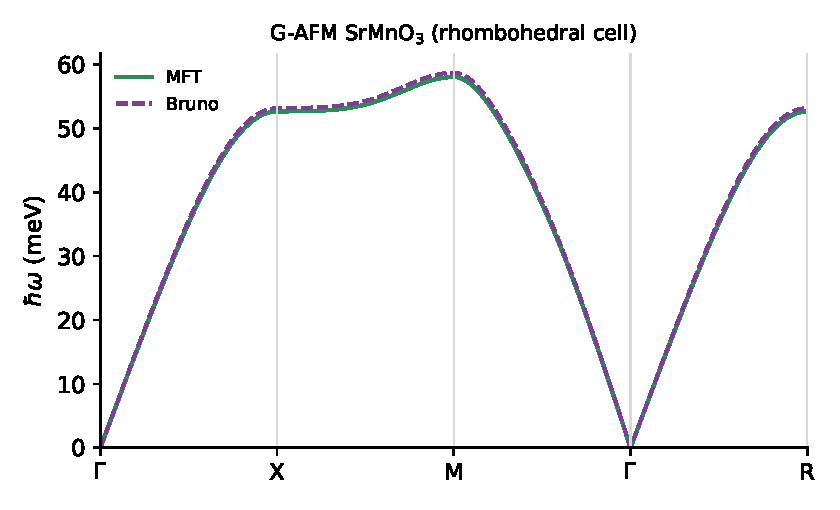
\includegraphics[width=\textwidth]{figs/srmno3_magnon.pdf}\\
\small G-type SrMnO$_3$: two degenerate Goldstone branches, linear at $\Gamma$; Bruno raises the zone-boundary energies slightly (insulator, $\omega\ll\Delta$).
\end{columns}
\end{frame}

% =====================================================================
\section{Parallel implementation}
% =====================================================================
\begin{frame}{MPI layout \src{parallel.py}}
\centering
\resizebox{0.86\textwidth}{!}{%
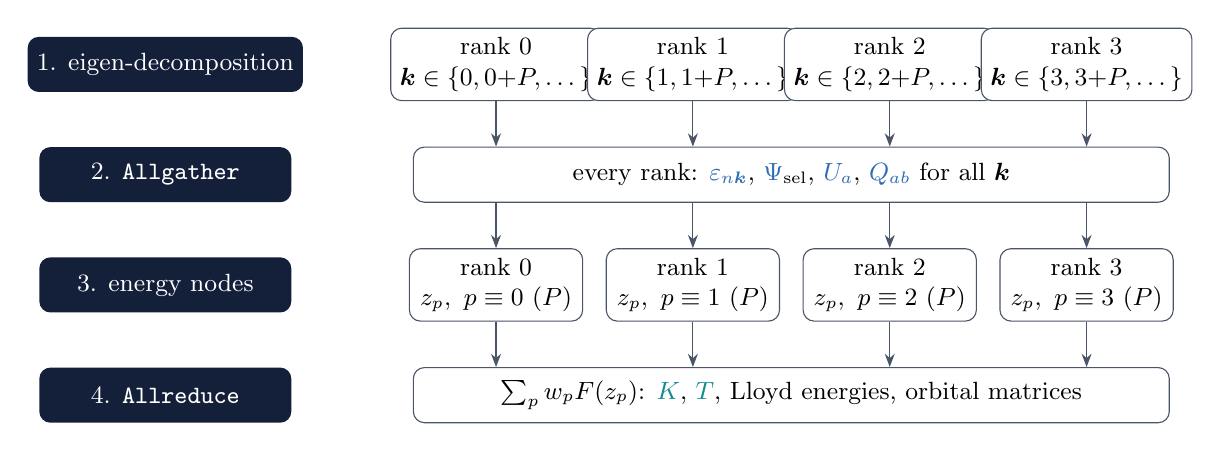
\begin{tikzpicture}[font=\small,
  r/.style={draw=cC,fill=white,rounded corners,minimum width=2.2cm,minimum height=7mm,align=center},
  ph/.style={draw=none,fill=navy,text=white,rounded corners,minimum width=3.2cm,minimum height=7mm}]
\node[ph] (p1) at (0,3) {1. eigen-decomposition};
\foreach \r in {0,1,2,3}{\node[r] (k\r) at (4.2+\r*2.5,3) {rank \r\\$\bm k\in\{\r,\r{+}P,\dots\}$};}
\node[ph] (p2) at (0,1.6) {2. \texttt{Allgather}};
\node[r,minimum width=9.6cm] (ag) at (7.95,1.6) {every rank: $\cG{\varepsilon_{n\bm k}}$, $\Psim_{\rm sel}$, $\cG{U_a}$, $\cG{Q_{ab}}$ for all $\bm k$};
\node[ph] (p3) at (0,0.2) {3. energy nodes};
\foreach \r in {0,1,2,3}{\node[r] (z\r) at (4.2+\r*2.5,0.2) {rank \r\\$z_p,\ p\equiv \r\ (P)$};}
\node[ph] (p4) at (0,-1.2) {4. \texttt{Allreduce}};
\node[r,minimum width=9.6cm] (ar) at (7.95,-1.2) {$\sum_p w_p F(z_p)$: $\K$, $\T$, Lloyd energies, orbital matrices};
\foreach \r in {0,1,2,3}{\draw[-Stealth,cC] (k\r)--(ag.north -| k\r); \draw[-Stealth,cC] (ag.south -| z\r)--(z\r); \draw[-Stealth,cC] (z\r)--(ar.north -| z\r);}
\end{tikzpicture}}\\[4pt]
\footnotesize
\begin{tabular}{lll}
\toprule
task & cost per energy node & parallel axis\\
\midrule
fast engine (on-site) & $N_k N_{\rm sel}^2N_b$ + FFT & $z$\\
weighted engine & $16\times N_kN_{\rm sel}^2N_b$ + 16 FFTs & $z$\\
Lloyd (per pair, angle) & $12\times N_kn^2N_b$ & $z$\\
MAE & $N_k$ diagonalisations per direction & $\bm k$\\
\bottomrule
\end{tabular}\quad
\begin{tabular}{l}
SrMnO$_3$, $5^3$: 34.6 s $\to$ 18.8 s (2 ranks)\\
results identical to $10^{-14}$\\
\texttt{OMP\_NUM\_THREADS=1}, 1 rank/core
\end{tabular}
\end{frame}

% =====================================================================
\section{Validation and results}
% =====================================================================
\begin{frame}{Exactness tests}
\begin{columns}[c]
\column{0.55\textwidth}
\small
\renewcommand{\arraystretch}{1.15}
\begin{tabular}{p{4.6cm}r}
\toprule
test (\texttt{tests/}) & max error\\
\midrule
GF Hessian vs.\ finite differences, cluster with SOC, AFM, spin-dependent hopping & $1.5\times10^{-7}$\\
weighted partition vs.\ finite differences & $1.3\times10^{-7}$\\
$k$-mesh/FFT vs.\ explicit supercell & $9\times10^{-16}$\\
Lloyd vs.\ exact $\Om$ (both partitions) & $2.5\times10^{-11}$\\
Goldstone sum rule (weighted) & $4\times10^{-15}$\\
Heisenberg round trip ($\J$, $\A$) & $7\times10^{-16}$\\
LSWT: FM, AFM chain, gap & analytic\\
real SrMnO$_3$: $\sum_{\bm R}\K$ vs.\ FD & $-66.571/-66.565$\\
\bottomrule
\end{tabular}
\column{0.43\textwidth}
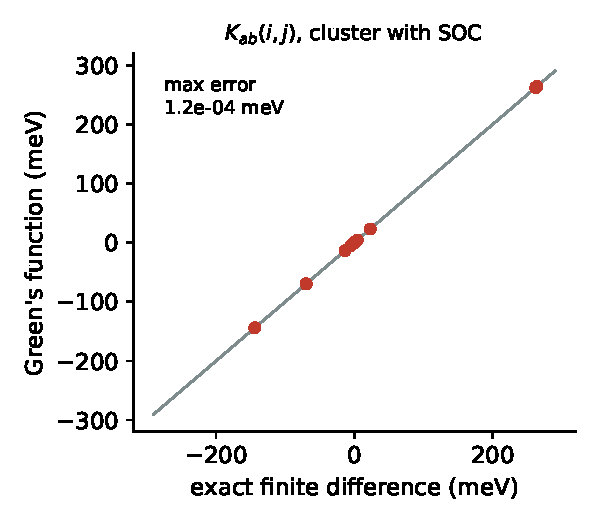
\includegraphics[width=\textwidth]{figs/parity.pdf}\\
\small finite-difference error ($h=10^{-3}$) dominates the residual.
\end{columns}
\end{frame}

\begin{frame}{SrMnO$_3$: comparison with TB2J}
\begin{columns}[c]
\column{0.5\textwidth}
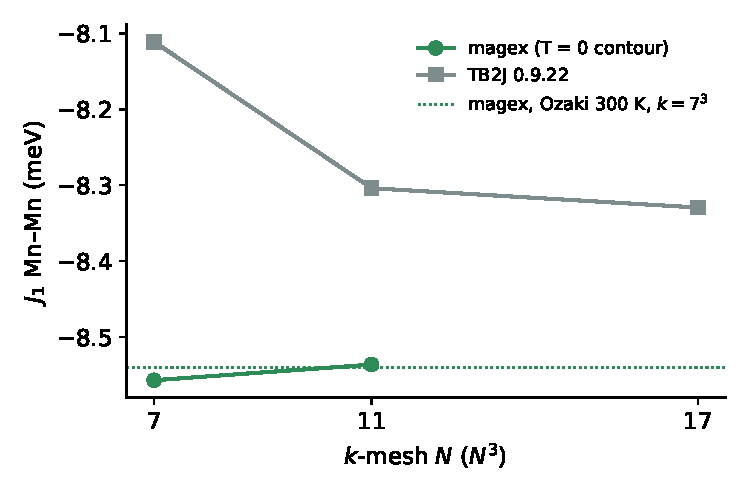
\includegraphics[width=\textwidth]{figs/srmno3_kconv.pdf}
\column{0.47\textwidth}
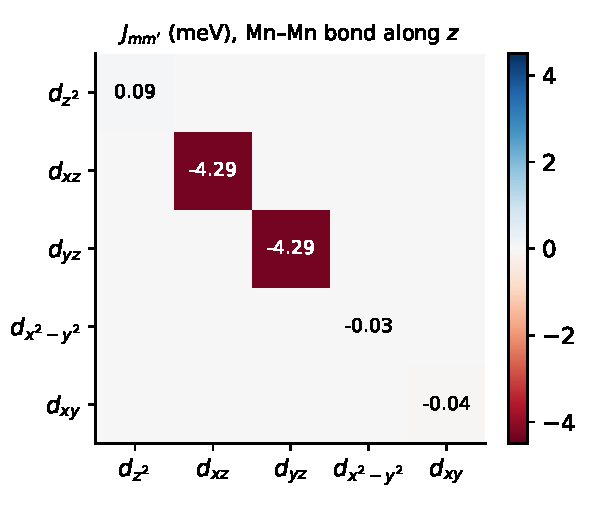
\includegraphics[width=0.9\textwidth]{figs/srmno3_orb.pdf}
\end{columns}
\small
\begin{itemize}
\item same Wannier data, on-site partition: magex $J_1=-8.54$ meV (converged at $7^3$), TB2J 0.9.22 $-8.33$ meV at $17^3$
\item $t_{2g}$ channel identical ($-4.291$ meV for $d_{xz}$, $d_{yz}$); the difference sits in the $e_g$ channel
\item magex matches brute-force energy differences of the same Hamiltonian to $10^{-4}$
\end{itemize}
\end{frame}

\begin{frame}{bcc Fe: the effect of rotational invariance}
\begin{columns}[c]
\column{0.58\textwidth}
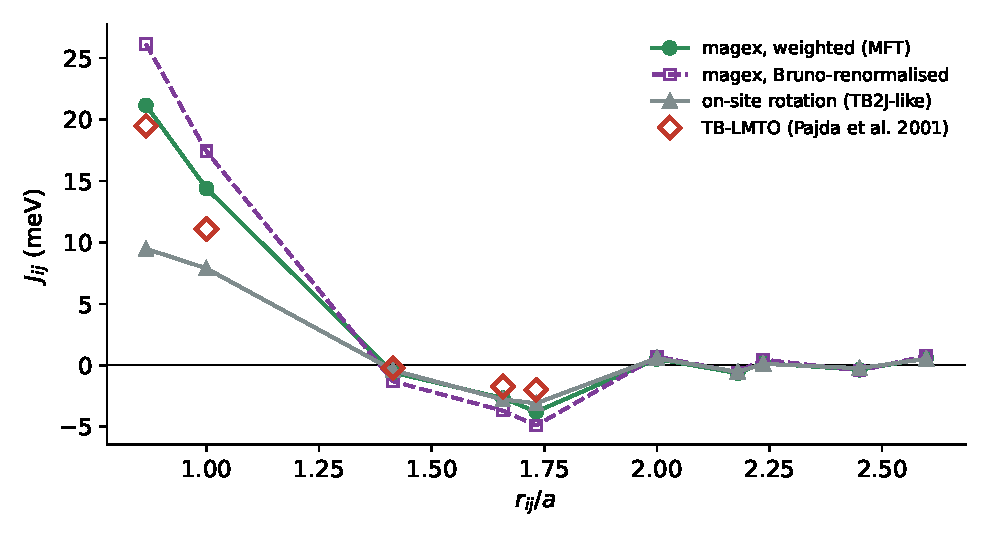
\includegraphics[width=\textwidth]{figs/fe_JR.pdf}
\column{0.4\textwidth}
\small
\renewcommand{\arraystretch}{1.2}
\begin{tabular}{lrr}
\toprule
 & $J_1$ & $T_{\rm MF}$\\
 & (meV) & (K)\\
\midrule
on-site (TB2J-like) & 9.5 & 441\\
\cH{weighted, MFT} & \cH{21.2} & \cH{1427}\\
weighted, Bruno & 26.1 & 1660\\
TB-LMTO (Pajda) & 19.5 & 1414\\
experiment & -- & 1043\\
\bottomrule
\end{tabular}\\[4pt]
$k_BT_{\rm MF}=\tfrac23\sum_j\cJ{J_{0j}}$\\[3pt]
QE + Wannier90 (s,p,d), $13^3$, 2 MPI ranks, 2.7 min.
\end{columns}
\takeaway{rotating the inter-atomic exchange field with the moment turns an unphysical Wannier result into LMTO-quality exchange.}
\end{frame}

\begin{frame}{bcc Fe: spin waves}
\begin{columns}[c]
\column{0.6\textwidth}
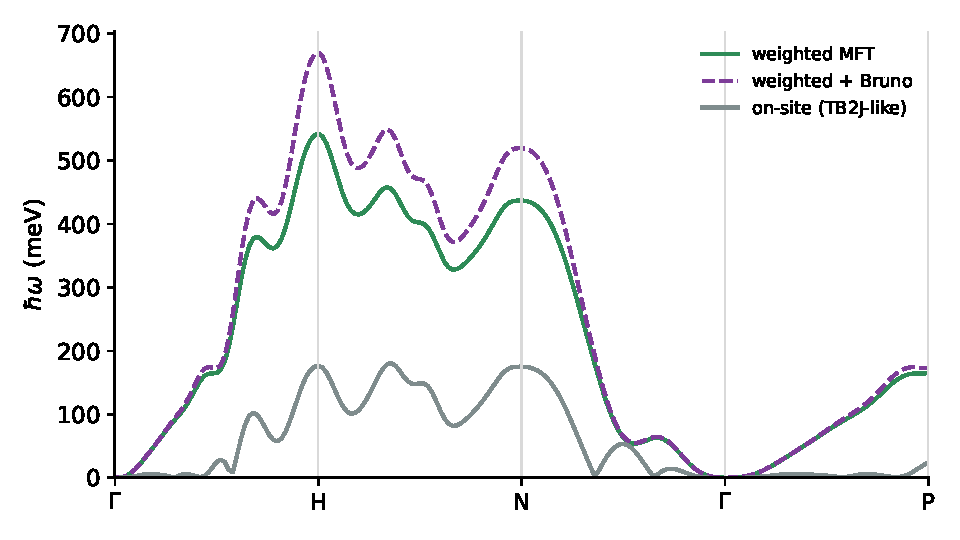
\includegraphics[width=\textwidth]{figs/fe_magnon.pdf}
\column{0.38\textwidth}
\small
\begin{itemize}
\item weighted MFT: maximum 542 meV at H, typical of LKAG Fe results
\item Bruno: zone-boundary energies up by $\sim$20\% where $\omega$ approaches $\Delta\approx2$ eV
\item on-site rotation: soft spectrum, consistent with $T_{\rm MF}=441$ K
\item the residual wiggles reflect the finite $13^3$ real-space range of $\J(\bm R)$
\end{itemize}
\end{columns}
\end{frame}

\begin{frame}{CrI$_3$: one run vs.\ three runs}
\begin{columns}[c]
\column{0.58\textwidth}
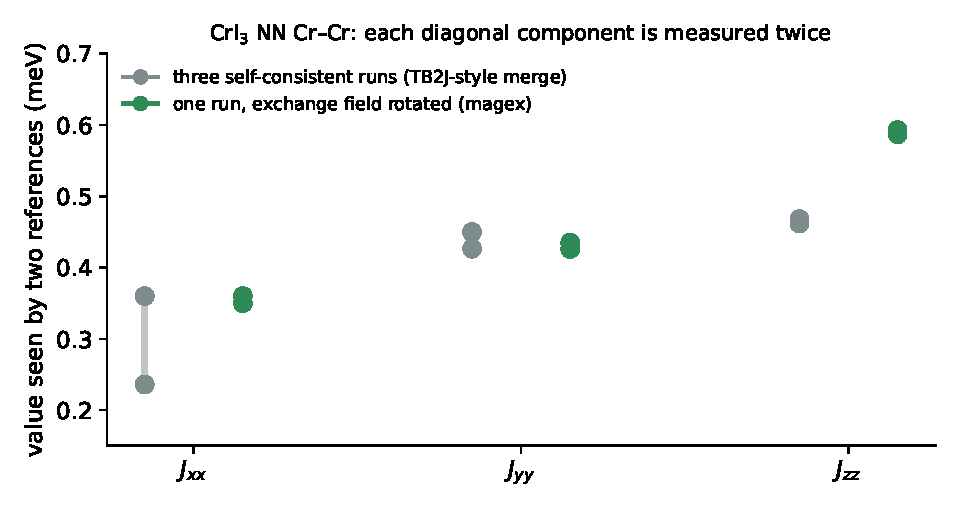
\includegraphics[width=\textwidth]{figs/cri3_consistency.pdf}
\column{0.4\textwidth}
\small
\begin{itemize}
\item TB2J example data: spinor VASP runs with spins along $x$, $y$, $z$ (rotated lattices)
\item every diagonal component is measured by two references
\item three separately Wannierised runs disagree by up to 35\% ($J_{xx}$)
\item one run with $\X$ rotated agrees with itself to 3\%
\item TR partner test ($\n\to-\n$): 1--5\%
\end{itemize}
\end{columns}
\takeaway{the single-run approach removes inter-run Wannier noise; for spinor input check the TR line, or use collinear $+$ atomic SOC.}
\end{frame}

% =====================================================================
\section{Using the code}
% =====================================================================
\begin{frame}[fragile]{Input and output}
\begin{columns}[T]
\column{0.5\textwidth}
\begin{plainbox}{cC}
\tiny
\begin{verbatim}
[input]
win = "wannier90.up.win"
hr_up = "wannier90.up_hr.dat"
hr_dn = "wannier90.dn_hr.dat"
centres = "wannier90.up_centres.xyz"
efermi = 4.327
[magnetic]
elements = ["Mn"];  ligands = ["O"]
[soc_xi]                  # optional atomic SOC
"Mn:d" = 0.045
[calc]
kmesh = [9, 9, 9]
partition = "weighted"    # or "onsite"
refs = "auto"             # x, y, z with SOC
mae = true
[magnon]
path = "GXMGR"
\end{verbatim}
\end{plainbox}
\column{0.47\textwidth}
\small
\texttt{mpirun -n 40 magex run in.toml}\\[4pt]
\textbf{exchange.out}: moments and charges, sum rule, $\J$ (MFT, Bruno, downfolded), $\Dv$, $\J^{\rm ani}$ with residuals, $\A_i$ and easy axes, Lloyd table, MAE with TR and Heisenberg checks, orbital-resolved $\J$, timings.\\[3pt]
\textbf{results.json}: all pairs in the supercell, full tensors.\\[3pt]
\textbf{pairs.csv}, \textbf{magnon\_band\_*.dat/png}.\\[6pt]
\begin{plainbox}{cS}
\small\textbf{Limitations:} frozen potential; collinear references; spinor input needs a near-real gauge; Bruno/downfolding act on the isotropic channel; no local-axis projections.
\end{plainbox}
\end{columns}
\end{frame}

\begin{frame}{Summary}
\begin{columns}[T]
\column{0.5\textwidth}
\begin{plainbox}{cH}
\small\textbf{Theory}
\begin{itemize}
\item exact force-theorem Hessians of $\Om$ for rotations of the exchange field
\item weighted partition $\Rightarrow$ exact rotational invariance
\item one Hamiltonian, three references $\Rightarrow$ $\J$, $\Dv$, $\J^{\rm ani}$, $\A$
\item Ozaki poles, Bruno, downfolding, Lloyd, LSWT
\end{itemize}
\end{plainbox}
\column{0.47\textwidth}
\begin{plainbox}{cJ}
\small\textbf{Results}
\begin{itemize}
\item machine-precision tests of every formula
\item bcc Fe: $J_1=21.2$ meV, $T_{\rm MF}=1427$ K (LMTO 19.5, 1414 K)
\item SrMnO$_3$ Heisenberg-like, Fe strongly non-Heisenberg at large angles
\item CrI$_3$: single-run tensors self-consistent to 3\%
\end{itemize}
\end{plainbox}
\end{columns}
\vspace{6pt}
\begin{plainbox}{cM}
\small\textbf{Next:} VI$_3$ and Pt/VI$_3$ magnons with SIA; CrSb (altermagnet) and interface exchange; self-consistent constrained references; GPU port of the weighted engine.
\end{plainbox}
\end{frame}

\end{document}
